\documentclass[12pt,a4paper]{report}

\usepackage[utf8]{inputenc}
\usepackage[T1]{fontenc}%encodage de la police
\usepackage[french]{babel}%langue française

\renewcommand{\thesection}{\arabic{section}} %changement du style de numérotation
\usepackage{graphicx}
\usepackage{geometry}
\usepackage{setspace} %line spacing d'un paragraphe
\usepackage{amsmath}
\usepackage{amssymb}
\usepackage{float}
\usepackage{mathrsfs}
\usepackage[most]{tcolorbox}
\usepackage{hyphenat} %encoder le '-'
\usepackage[most]{tcolorbox}
\usepackage{hyperref}
\usepackage{float} %position des tableaux
\restylefloat{table}
\usepackage{pgfplots}
\usepackage{listings}
\usepackage{tikz}
\usetikzlibrary{calc}
\usepackage{tocloft}
\usepackage{listings}

\usepackage{caption,subcaption}
\usepackage[showframe]{geometry}

\hyphenation{he-lio-trope opos-sum} 
\usepackage{xcolor}
\usepackage{listings}


% le niveau de détails de sous-sections qu'on veut 
\setcounter{tocdepth}{4}
\setcounter{secnumdepth}{4}

\newtcblisting{commandshell}{colback=black,colupper=white,colframe=yellow!75!black,
listing only,listing options={language=sh},
every listing line={\textcolor{green}{\small\ttfamily\bfseries \$ }}}

\lstset{basicstyle=\ttfamily,
  showstringspaces=false,
  commentstyle=\color{red},
  keywordstyle=\color{blue},
  breaklines=true,
}




\begin{document}



\begin{titlepage}
	\centering
	
\includegraphics[scale=0.15]{figures/logotp.png}\par\vspace{2.5cm}
	{\scshape\Large Master 1 Informatique - TER\par}
	\vspace{1.5cm}
	{\huge\bfseries Système de reconnaissance d'individus pour une espèce de baleines noires en danger d'extinction \par}
	\vspace{1.5cm}
	{\Large\itshape Hugo Maitre \par}
	{\Large\itshape Thomas Lecampion \par}
	{\Large\itshape Adrien Linares \par}


\vspace{1em}

	\vfill
	Encadrant:\par
	Pr. William \textsc{Puech}\par
	\vfill
	
	\vspace{1em}
	
% Bottom of the page
	{\large \today\par}
\end{titlepage}

% SOMMAIRE
\setlength{\cftbeforetoctitleskip}{-50pt} %remonter le toc
\begin{spacing}{1.2}
   \tableofcontents
\end{spacing}
 %\renewcommand{\contentsname}{Sommaire} change le titre de ToC
% FIN SOMMAIRE

\newpage

\section{Préambule}
\begin{spacing}{1.5}
\subsection{Contexte général}
Les baleines noires de l’Atlantique Nord sont une espèce de cétacés qui se distinguent des autres espèces de baleines entre autres par des callosités blanches se trouvant sur leurs têtes, qui est en fait de la peau kératinisée. Cette espèce de baleine, comme son nom l'indique, vit dans l'Océan Atlantique et à plus forte raison entre les degrés 20 et 60 de latitude Nord avec des déplacements variant selon les saisons.

% Zone d'habitat de la baleine noire de l'AN
\begin{figure}[H]
\begin{center}
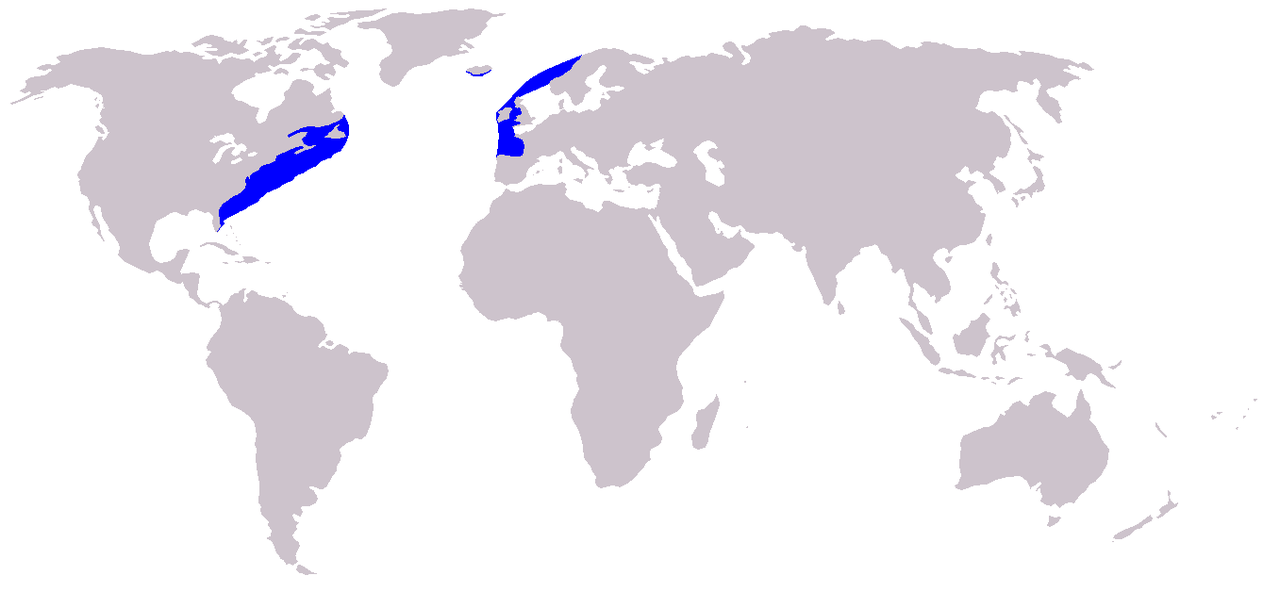
\includegraphics[scale=0.30]{figures/repartition.png}
\caption{Répartition géograpgique de l'espèce}
\end{center}
\end{figure}

Elles sont connues pour leurs comportements sociable vis à vis de l’humain. Elle se déplace lentement et souvent à la surface de l’eau. On estime qu’entre 1991 et 2007, 50\% des mortalités seraient dues à des collisions avec les bateaux\cite{WinNT}. Elle est également chassée principalement pour son huile, ce qui fait d'elle l'une des grandes baleines les plus menacées au monde. Aujourd’hui, sa population est estimée à moins de 450 individus, elle est clasifiée par l’IUCN\footnote{Union internationale pour la conservation de la nature} comme en danger critique d’extinction.

% Statut de conservation de cette espèce
\begin{figure}[H]
\begin{center}
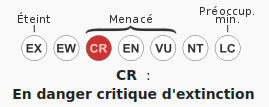
\includegraphics[scale=0.60]{figures/statut_conservation.png}
\caption{Statut de conservation établi par l'IUCN}
\end{center}
\end{figure}

C’est dans ce contexte que la NOAA (National Oceanic and Atmospheric Administration) a proposé un challenge d’une valeur de \$10.000 en 2016, afin de construire un système de reconnaissance automatique de ces baleines à partir de méthodes de machine learning. En effet, seulement quelques personnes dans le monde savent aujourd’hui distinguer ces baleines à l’œil nu, la majorité étant des chercheurs expérimentés dans le domaine. C’est de plus un processus qui prend beaucoup de temps. Cet outil sera donc nécessaire pour surveiller bien plus aisément la population de baleines noires de l’Atlantique Nord et de même avoir accès à son historique de santé. Le challenge a été publié sur Kaggle, site web rassemblant une communauté de data scientists et professionnels de l’apprentissage automatique, leur permettant de participer à des concours sur des problèmes réels, à partir de données réelles.
L'abréviation AN sera utilisée dans la suite de ce rapport pour \og Atlantique Nord \fg{}.
\subsubsection{Données}

Nous avons à notre disposition 11468 images aériennes de baleines noires de l’A.N. 
La qualité des images est très aléatoire, on constate par exemple des images 200*200 pixels côtoyant des images de très haute définition, images de 4000*3000 pixels. L’exposition des images est aussi très aléatoire même si l’on constate que 90\% des images sont correctement exposées. Certaines images souffrent de contraste trop fort ou inversement apparaissent trop “lisses”. On peut voir ci-dessous ces écarts sur un échantillon non aléatoire du dataset.

\newpage

\begin{figure}[H] % "[t!]" placement specifier just for this example
\begin{subfigure}{0.55\textwidth}
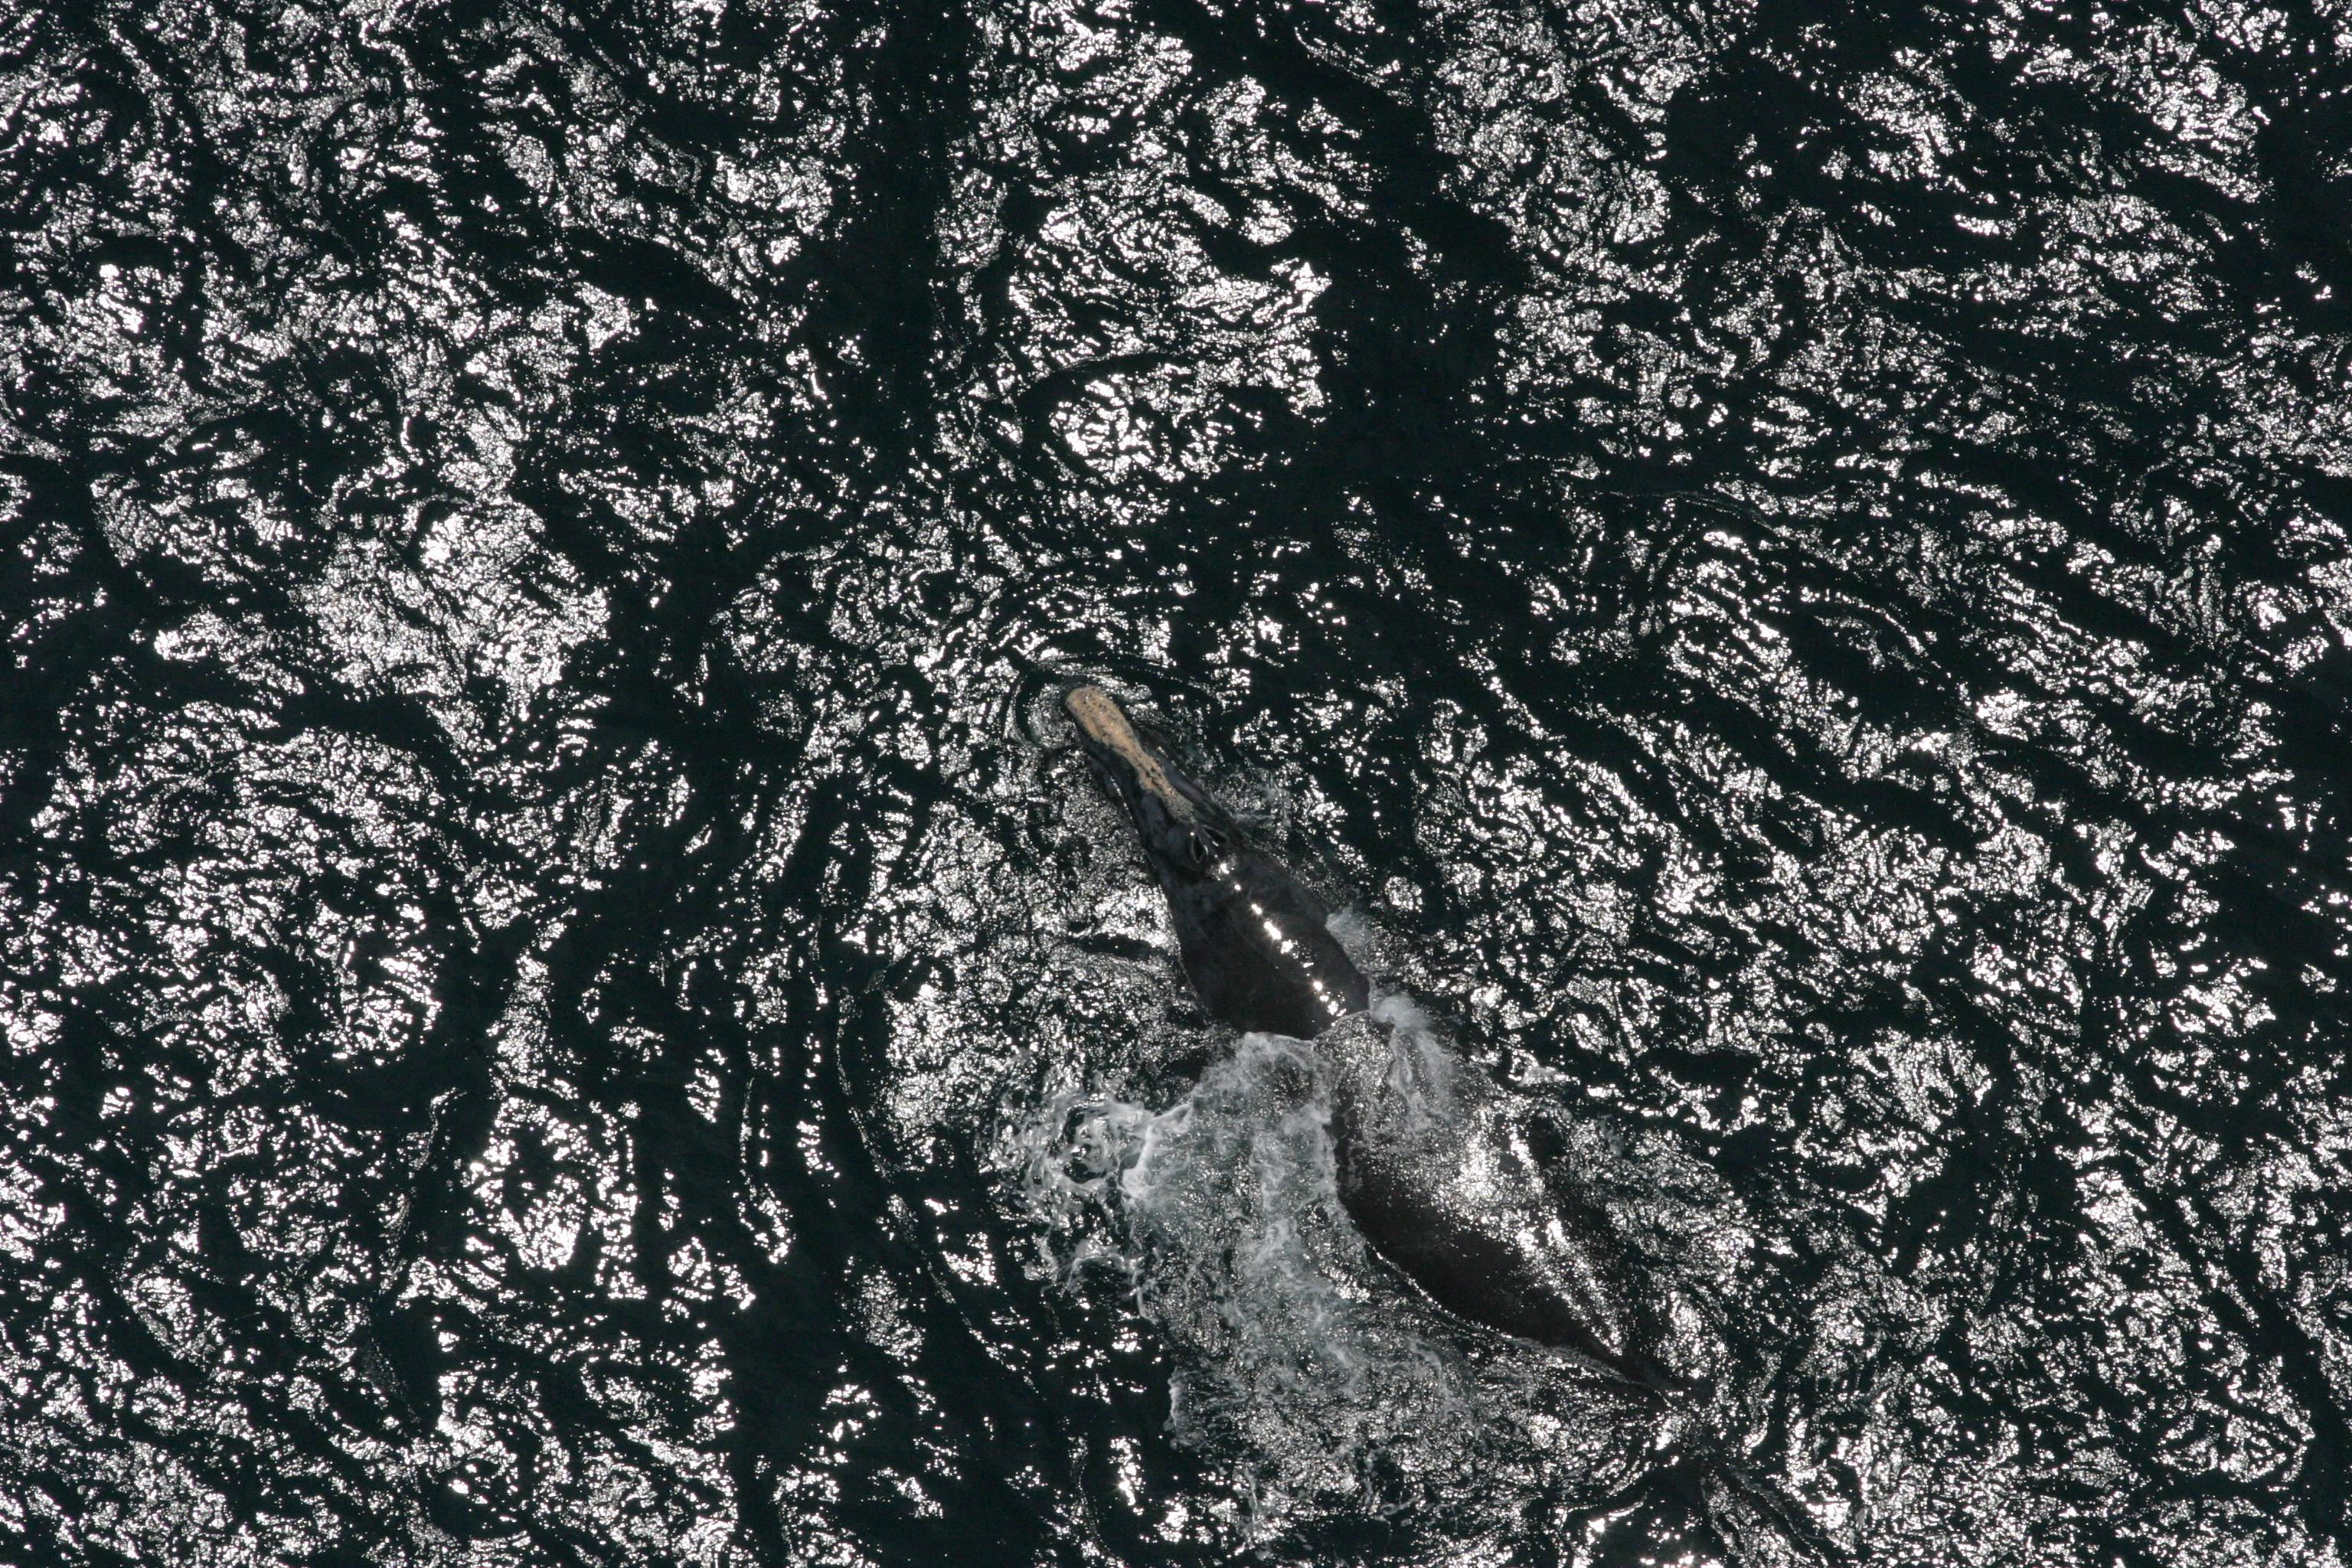
\includegraphics[width=\linewidth]{figures/whalesImg/w1.jpg}
\end{subfigure}\hspace*{\fill}
\begin{subfigure}{0.55\textwidth}
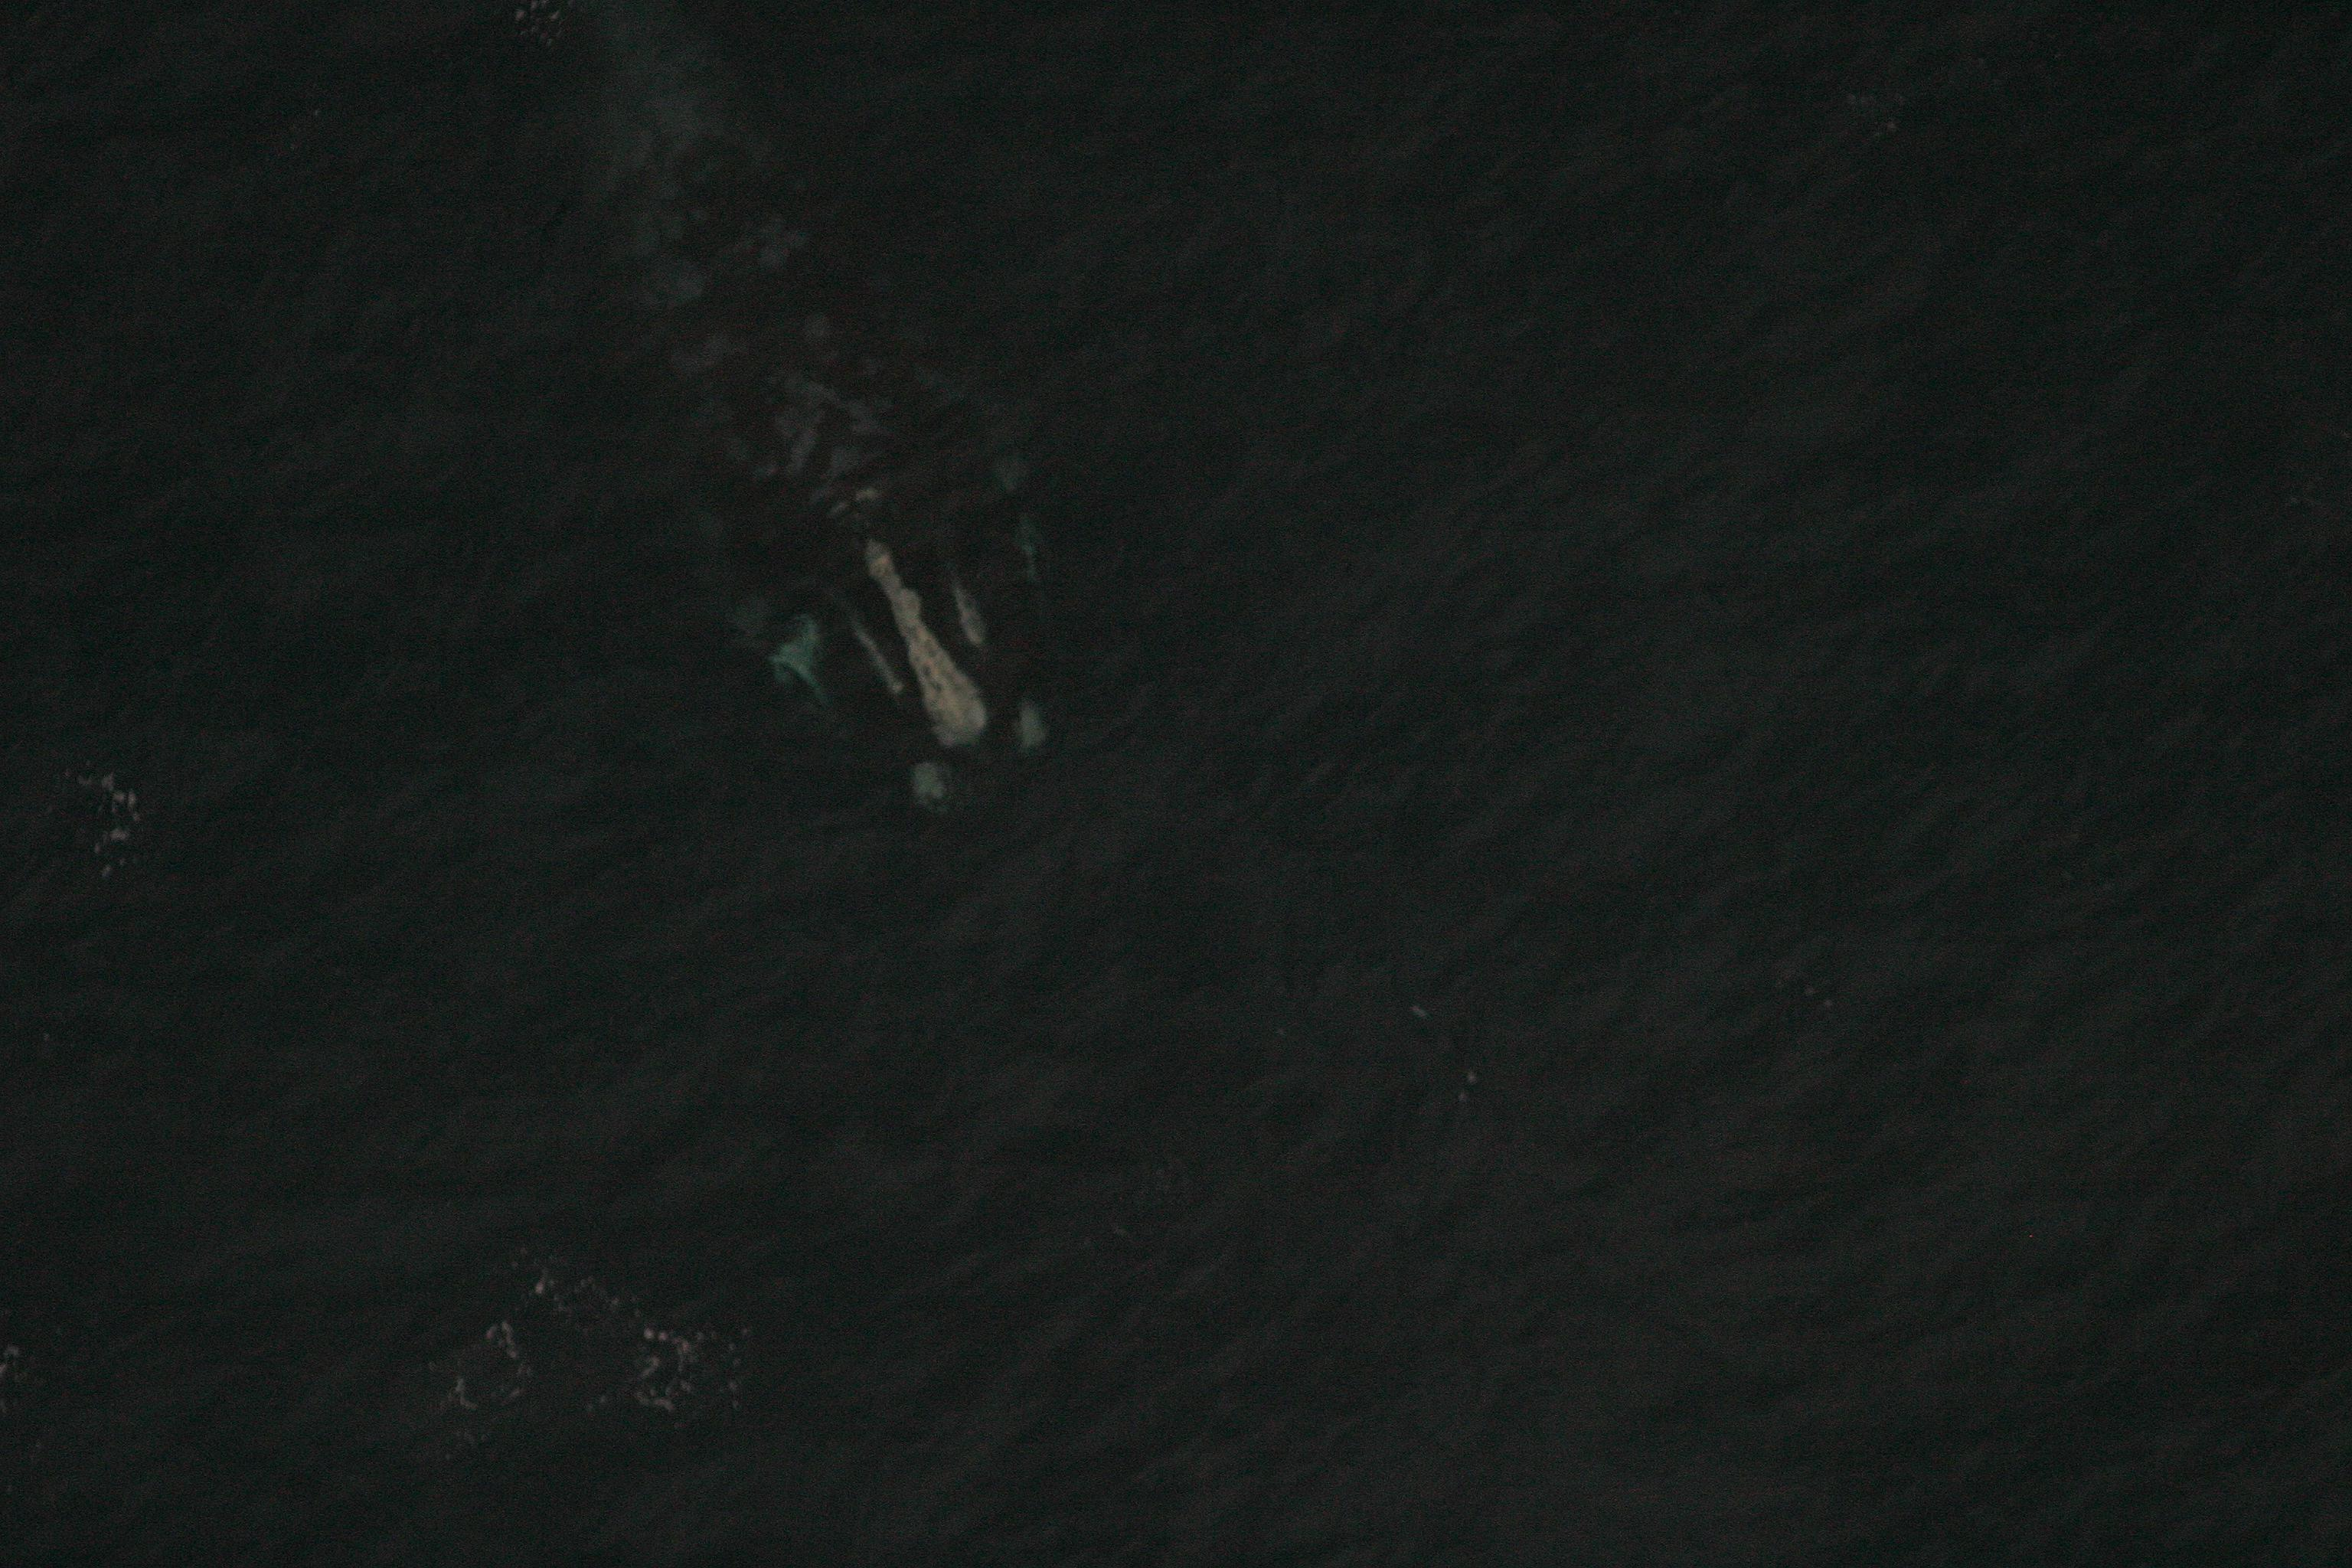
\includegraphics[width=\linewidth]{figures/whalesImg/w2.jpg}
\end{subfigure}

\medskip
\begin{subfigure}{0.55\textwidth}
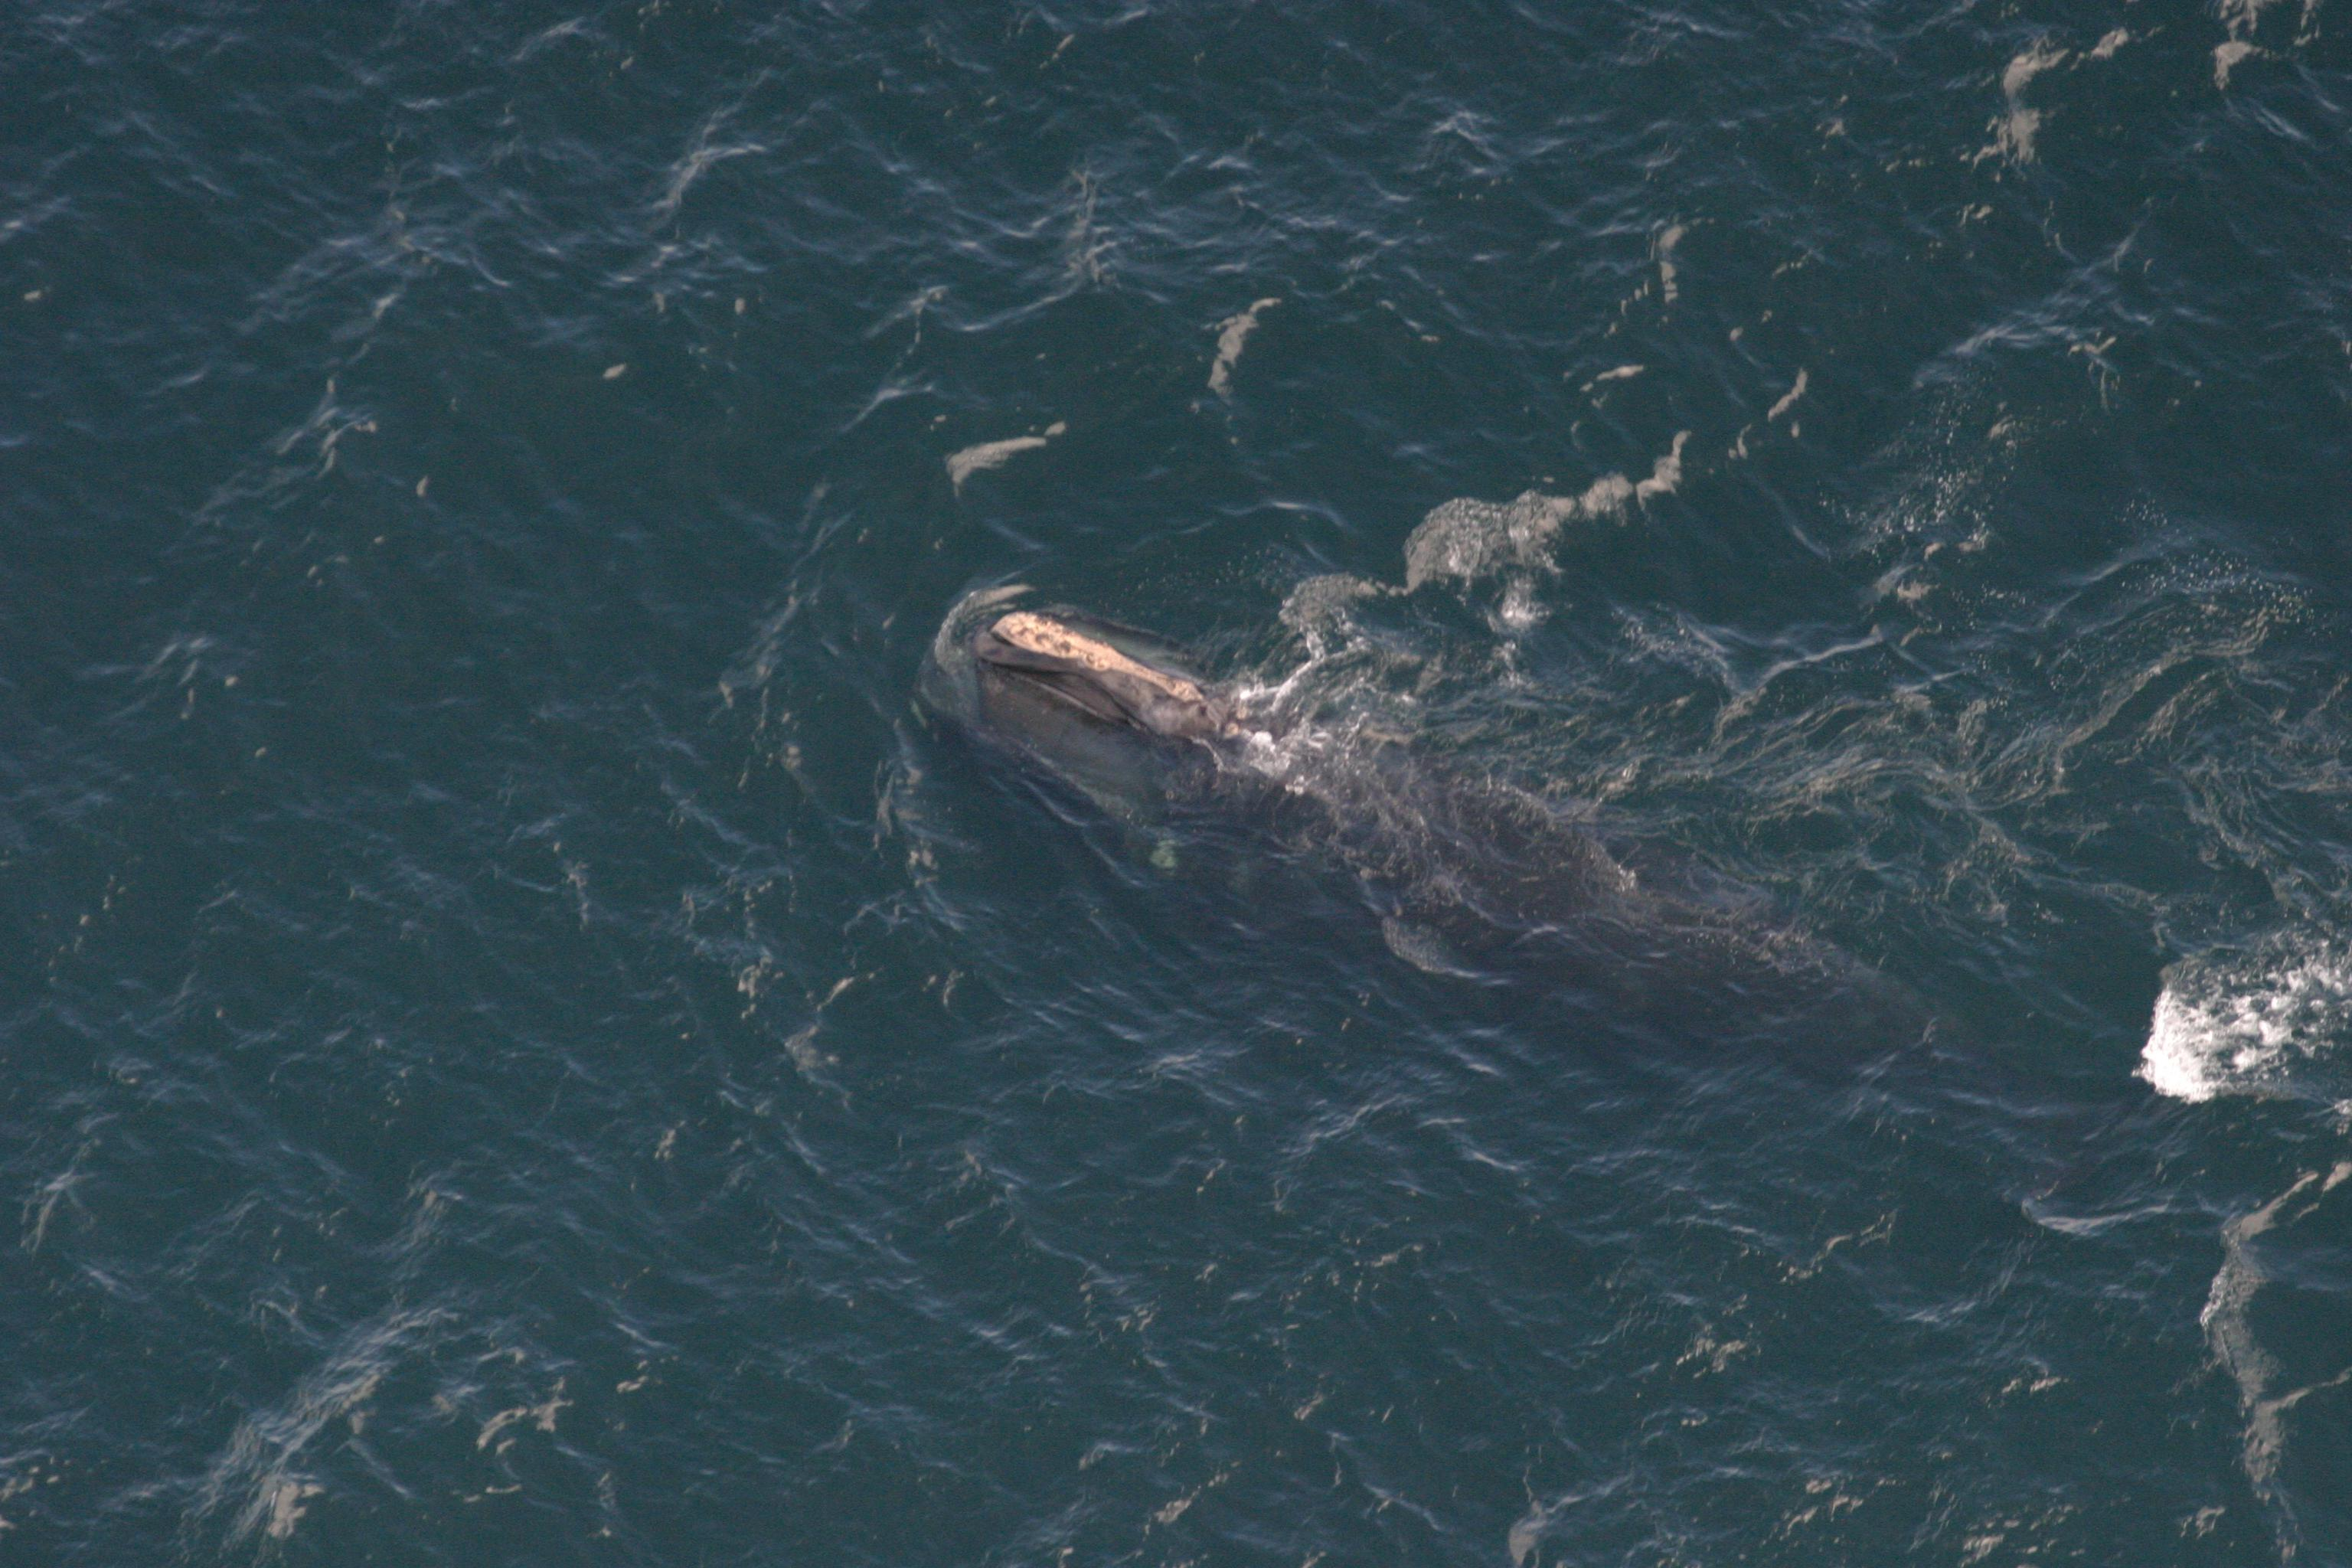
\includegraphics[width=\linewidth]{figures/whalesImg/w3.jpg}
\end{subfigure}\hspace*{\fill}
\begin{subfigure}{0.55\textwidth}
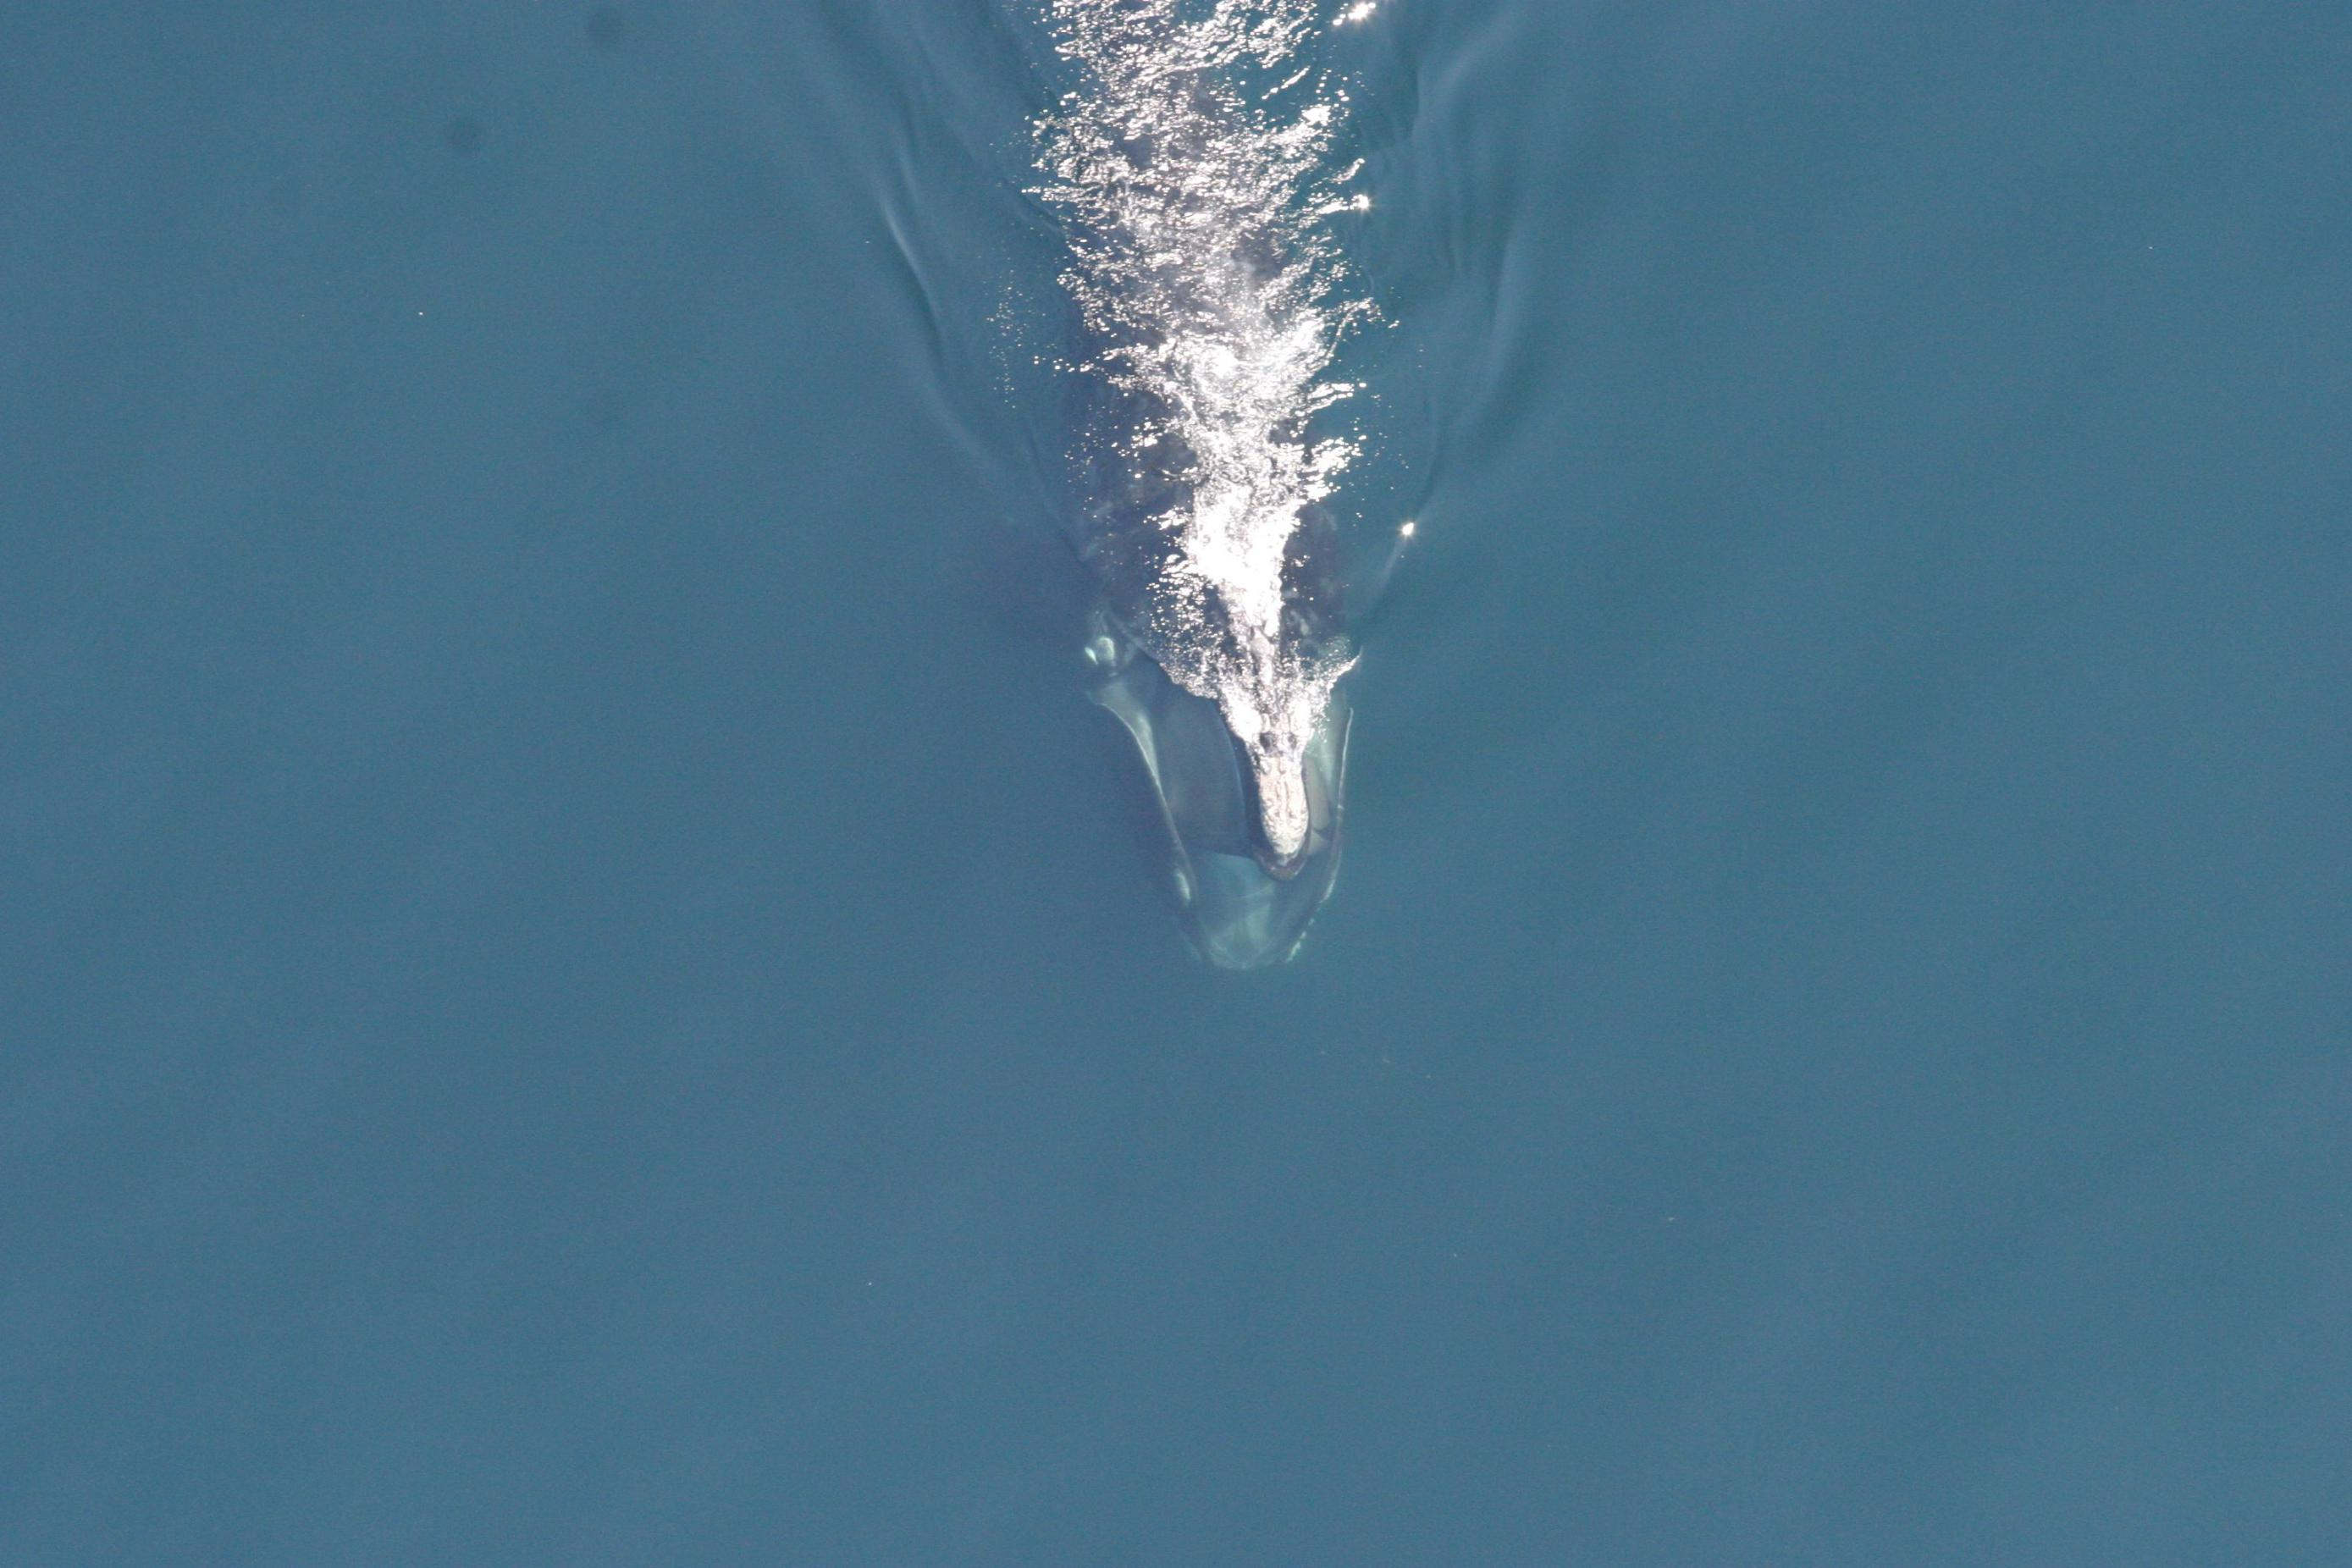
\includegraphics[width=\linewidth]{figures/whalesImg/w4.jpg}
\end{subfigure}

\medskip
\begin{subfigure}{0.55\textwidth}
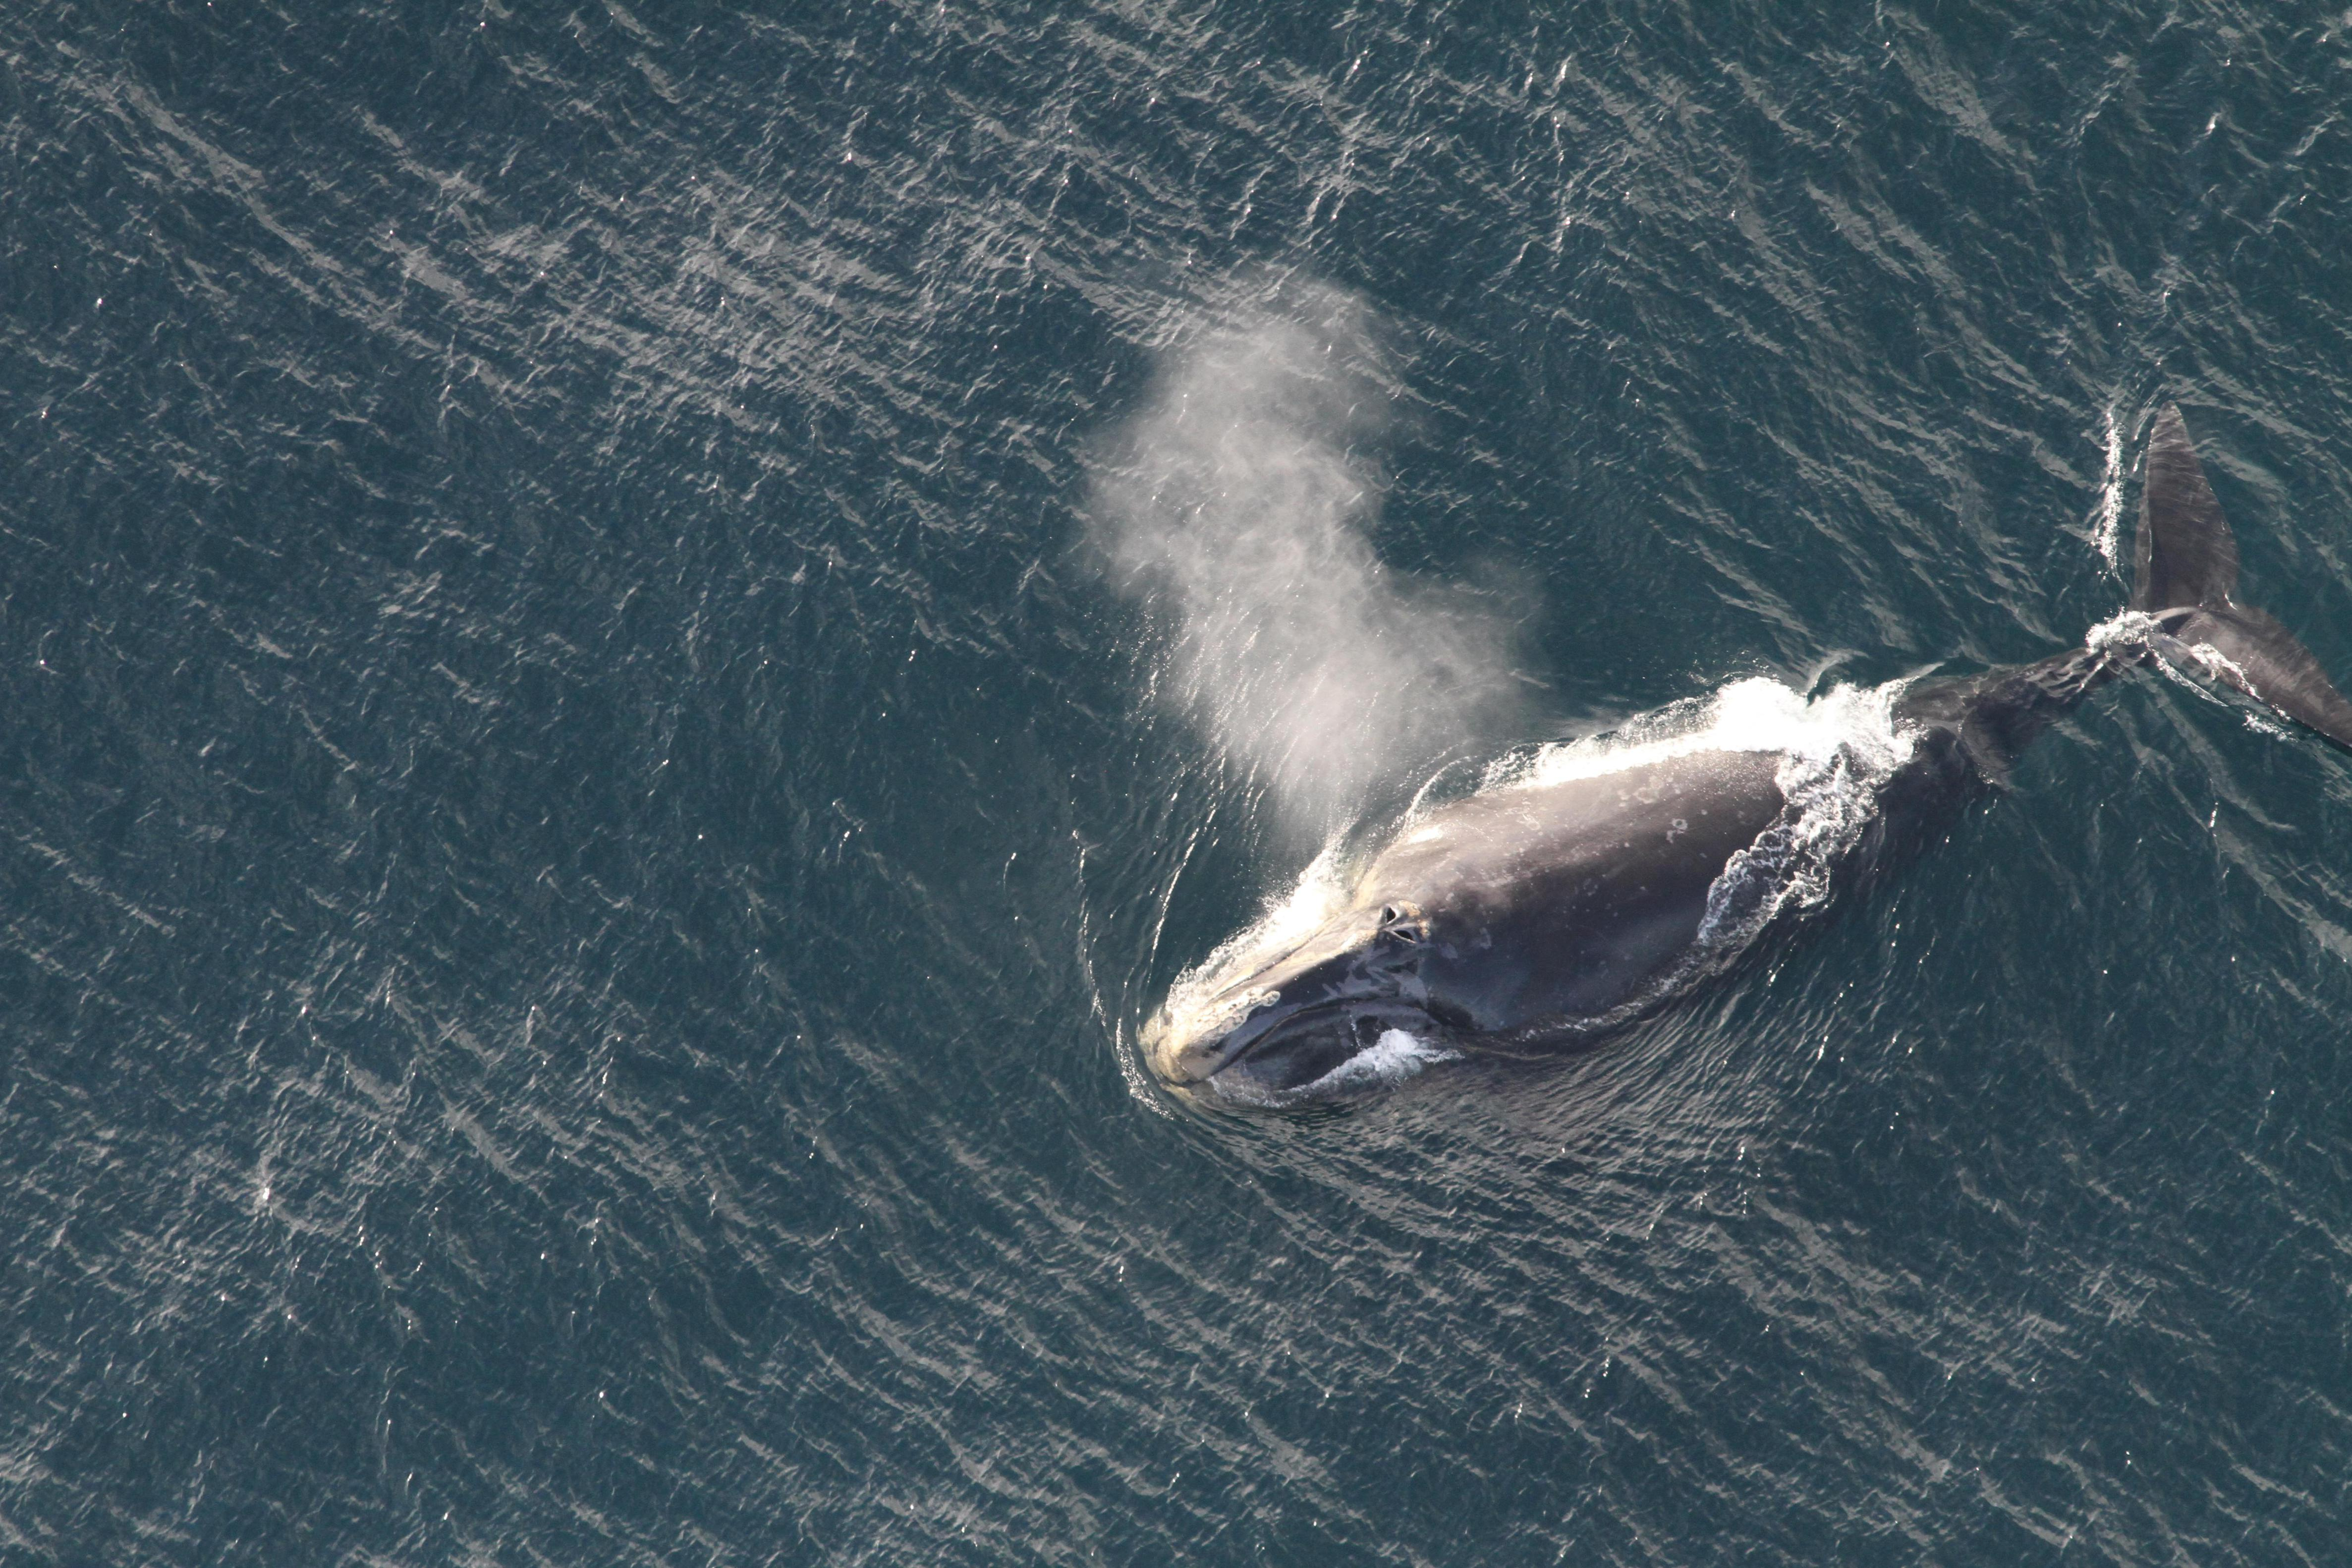
\includegraphics[width=\linewidth]{figures/whalesImg/w5.jpg}
\end{subfigure}\hspace*{\fill}
\begin{subfigure}{0.55\textwidth}
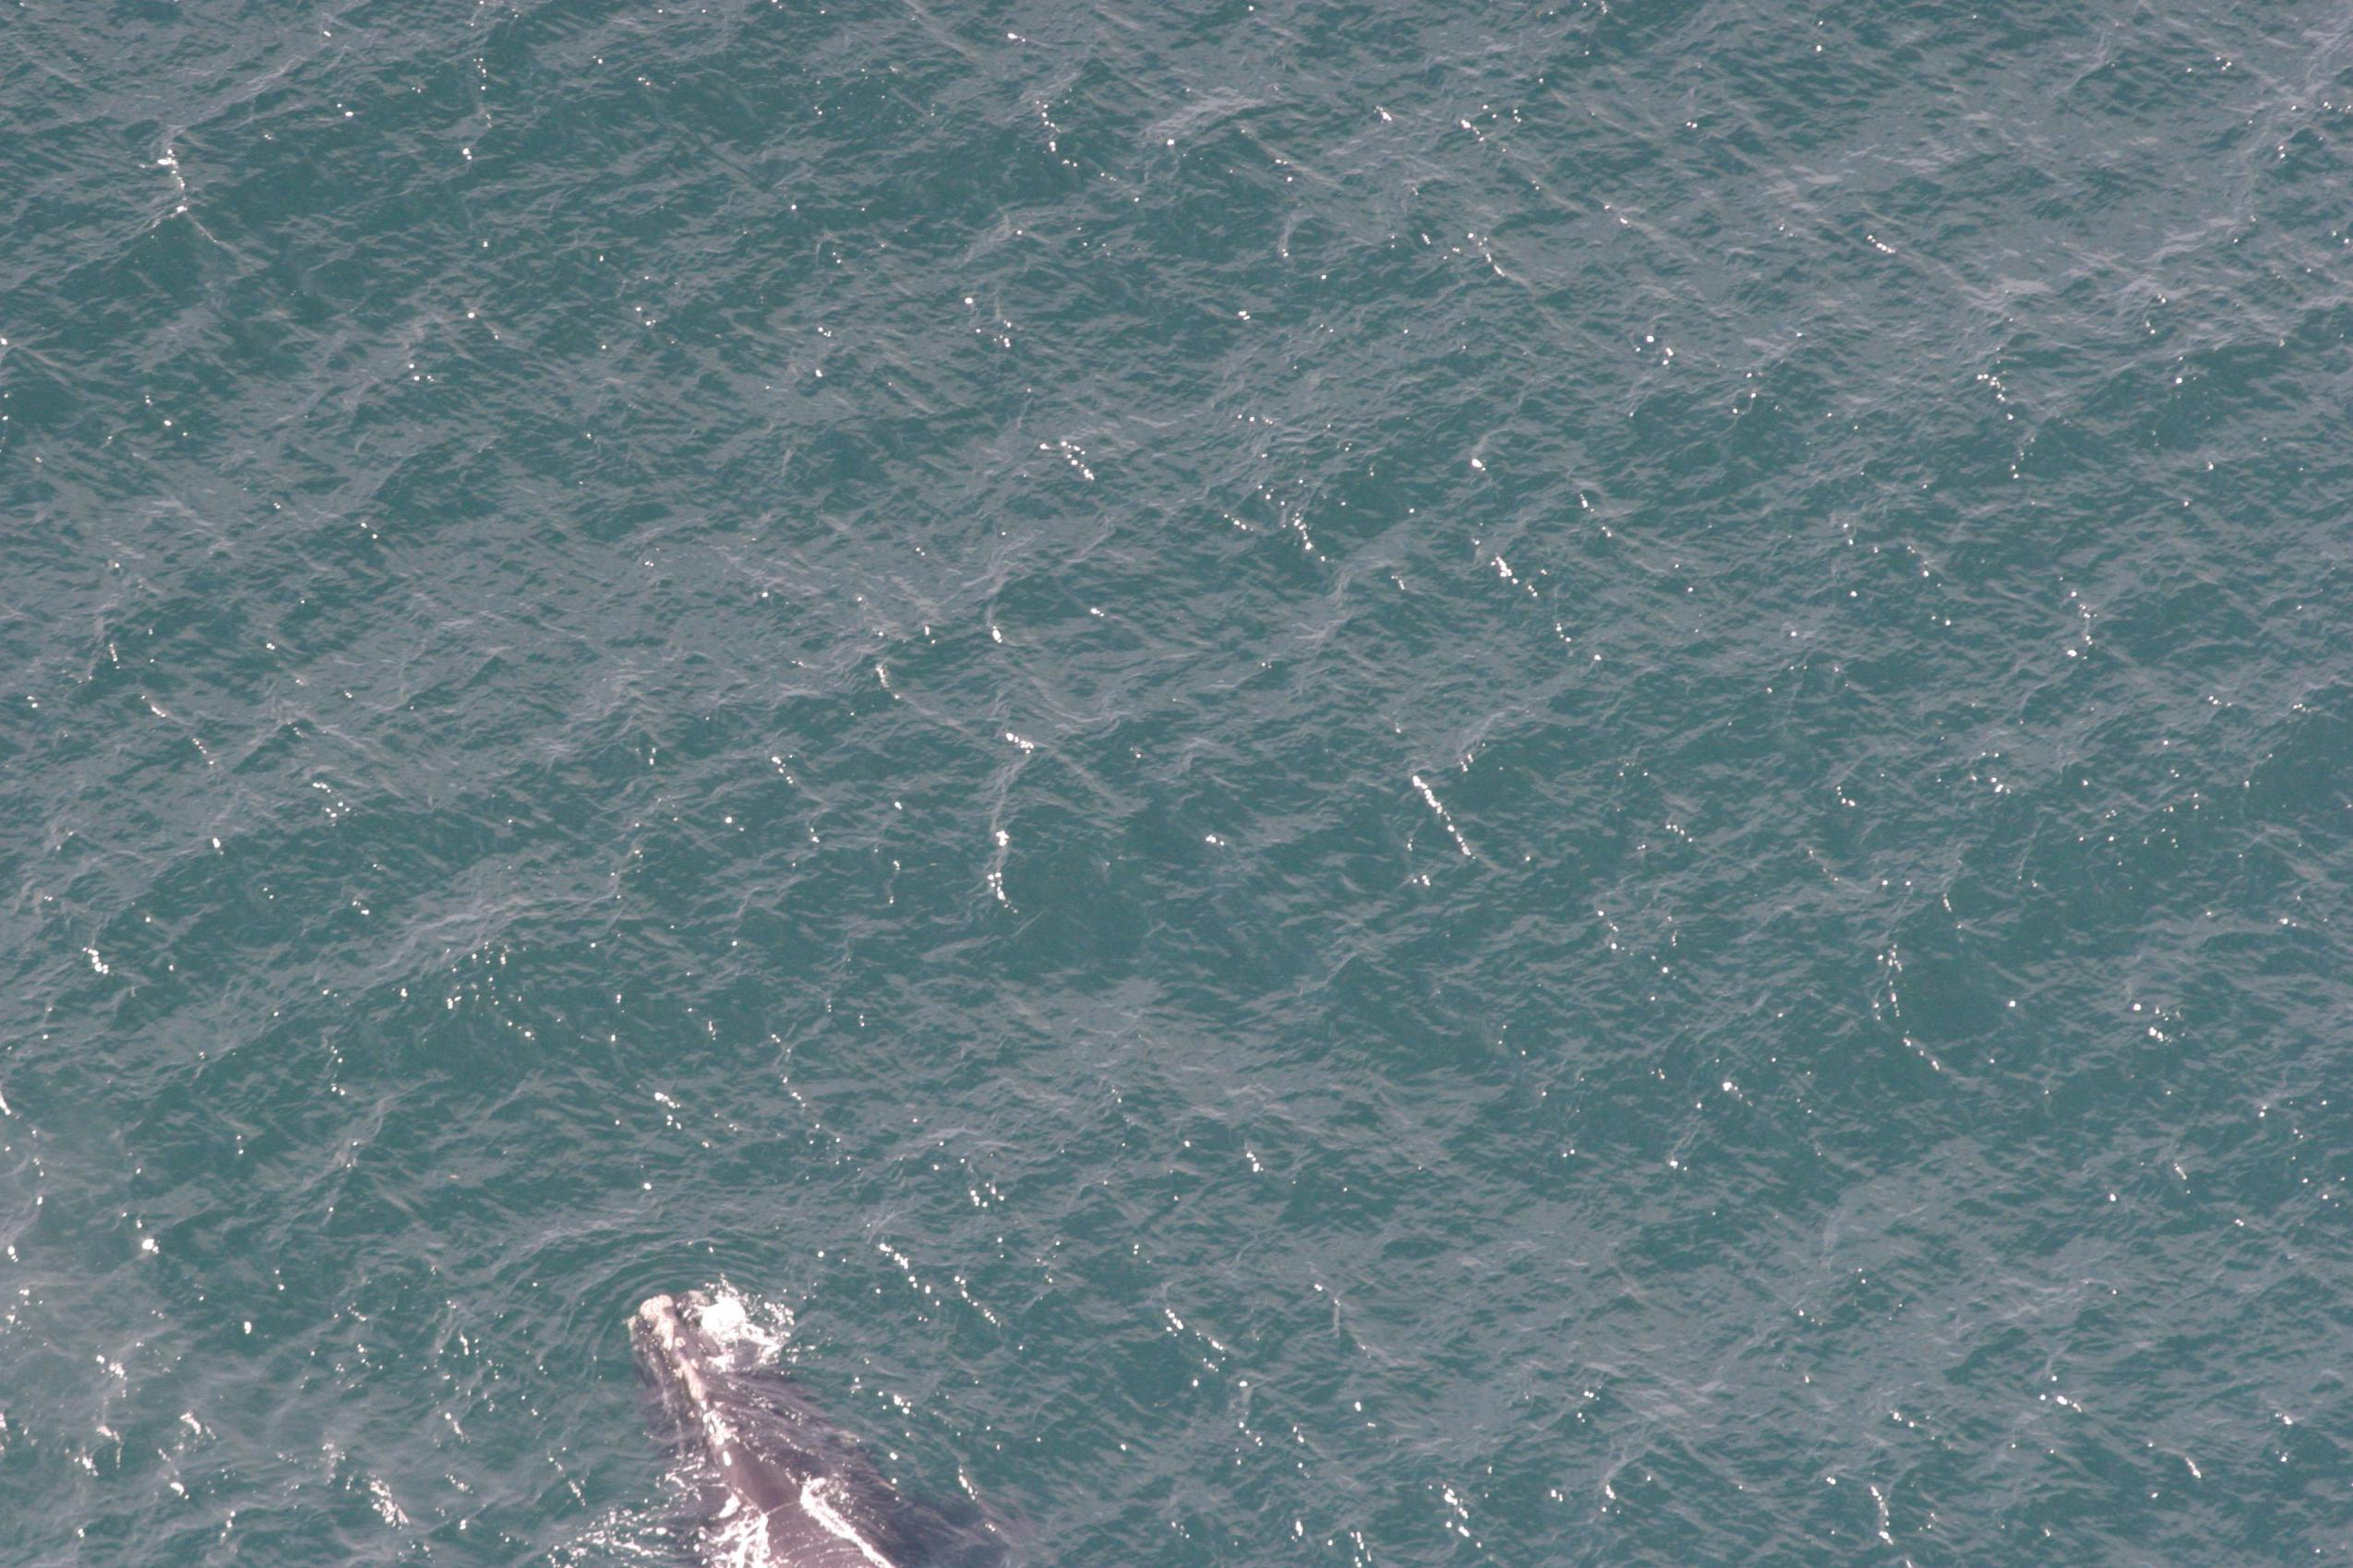
\includegraphics[width=\linewidth]{figures/whalesImg/w6.jpg}
\end{subfigure}

\caption{Echantillon non aléatoire du Dataset} \label{fig:1}
\end{figure}

\newpage

Parmi le dataset nous avons seulement 4544 images qui sont labellisées, c'est-à-dire environ 40\% du dataset. Nous n’avons bien évidemment pas accès aux labels des images restantes qui serviront à évaluer les performances de notre classifieur lors de la soumission de nos prédictions en ligne sur kaggle. On comprend déjà la difficulté qui nous attend: le manque de données.
On compte 447 individus de baleines noires répertoriées ce qui est probablement très proche du nombre de baleines noires de l’A.N existantes. Parmi les images labellisées on constate un nombre très hétérogène d’images attitrées à nos baleines. En effet certaines d’entre elles sont des “célébrités” ayant une cinquantaine d’images rien que pour elle mais la majorité des individus ont seulement entre 1 et 10 images. 

\begin{figure}[H]
\begin{center}
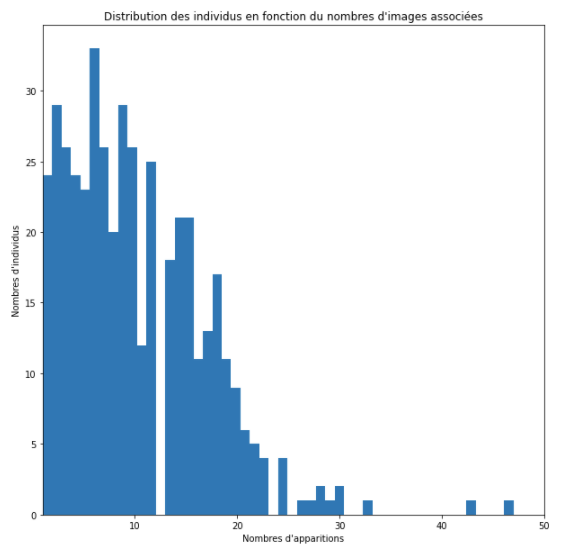
\includegraphics[scale=0.55]{figures/histo_appearance.png}
\caption{Visualisation de l'hétérogéneité des occurences}
\end{center}
\end{figure}




\subsubsection{Résultat attendu par Kaggle}
La solution s’imposant assez naturellement pour ce type de problème est d’utiliser une série de réseaux de neurones convolutifs.
La plateforme met à notre disposition une "vérité terrain" c’est-à-dire l'identité de 4544 images et nous évaluera sur les prédictions effectuées sur les 6924 images restantes.
La plateforme de Kaggle nous évaluera à la fin sur la précision, f1-score et rappel de notre modèle. À titre d’exemple, le modèle ayant le mieux performé est d'environ  80\%\cite{bogucki2019applying}.



\subsection{Organisation du travail} 

\subsubsection{Gestion de projet}

Nous avons eu l’idée de nous servir de Miro, outil collaboratif de travail mais qui a été au final très peu utilisé. En ce qui concerne la méthodologie de gestion de projet, nous avons choisi la méthode agile qui nous a semblé la plus adaptée ici.
Cette dernière a un usage plus particulier dans le contexte du deep learning et celui plus général du machine learning ............
La communication et les réunions se font sur Discord ou en présentiel.
Les rôles au sein de notre équipe ont été définis comme suit : \\
\begin{itemize}
% Mettre data analyst, ml engineer, data scientist... à la place de juste dév?
    \item \textbf{Hugo Maître} : chef de projet et développeur 
    \item \textbf{Adrien Linares} : développeur
    \item \textbf{Thomas Lecampion} : développeur
\end{itemize} 

\subsubsection{Plannification des tâches et planning}

% INCLURE TRELLO UNE CAPTURE?
Afin de mener à bien ce projet, nous avons utilisé différents outils nécessaires à l’organisation des tâches et de l’avancement dans le temps du projet. Nous avons premièrement utilisé Gantt, qui était avant tout un planning prévisionnel, dont voici ci-dessous une capture:

\begin{figure}[H]
\begin{center}
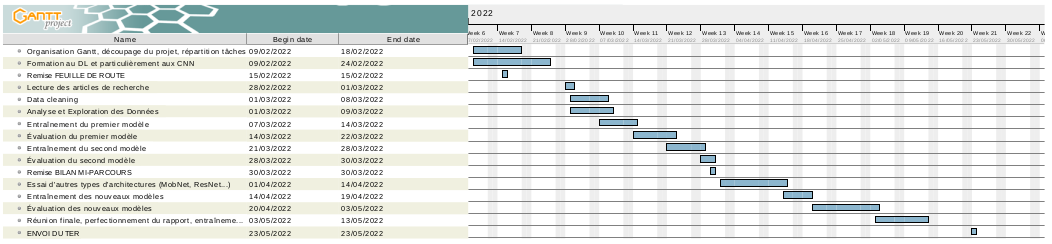
\includegraphics[scale=0.44]{figures/ganttTER.png}
\caption{Planning prévisionnel}
\end{center}
\end{figure}

\subsection{Motivations}
Nous avons recueilli les témoignages de chacun d'entre nous afin de savoir pourquoi nous avons, à l'uninanimité, choisi un tel projet et pas un autre.

\vspace{1em}

\begin{itemize}

\item \textbf{Thomas Lecampion:} J’ai choisi de rejoindre mes collègues sur ce TER pour m’initier au machine learning. En effet, c’est un domaine dans lequel je n’ai littéralement aucune expérience avant l’affectation des sujets. Je souhaitais apprendre pour réaliser certains projets personnels. \\

\item \textbf{Adrien Linares:} Ce projet m’a semblé le compromis idéal sur des choses que j'affectionne particulièrement, d’une part, la protection de la biodiversité, de l’autre, le domaine du deep learning et du traitement d’images. Il me servira en effet de tremplin pour de futurs stages et emploi en m’apprenant davantage sur ces domaines. 
  \\

\item \textbf{Hugo Maître:} À remplir \\

\end{itemize}
En complément de ce qui a été dit, nous avions également hésité avec un autre projet portant sur du NLP mais le voyant déjà en cours nous avons choisi de faire quelque chose de nouveau, portant donc sur le Computer vision cette fois-ci.

\end{spacing}
\begin{spacing}{1.5}

\subsection{Difficultés majeures}
Dès le commencement, nous avons pu distinguer sur le projet trois difficultés majeures:


Premièrement, il est nécessaire d’uniquement récupérer les informations pertinentes sur chacune des images de notre dataset, isoler les baleines. Autrement dit, il nous faut un moyen de localiser et récupérer la zone autour d’une baleine présente sur une image. La difficulté à première vue réside dans le fait que les baleines sont prises sous différents angles de vues plus ou moins loin et n’occupe donc pas du tout le même espace sur l’image. Pour cela nous envisageons d’entraîner un réseau de neurones (certainement un des modèles YOLO) capable de  détecter automatiquement des objets sur une image. Une fois la baleine détectée et isolée il faudra certainement établir un deuxième réseau de neurones capable de reconnaître les différentes caractéristiques de la baleine probablement la tête et l’évent. Là aussi en regardant un petit peu nos images on s’aperçoit que l’écume blanche sur les images va grandement complexifier notre tâche puisque l’évent\footnote{narine double des cétacés } ou le bout de la tête sont des zones qui apparaissent aussi blanches comme l’écume aussi bien qu'il est parfois difficile même pour un humain de les repérer correctement sur l'image. De plus, les baleines peuvent se présenter sous différents profils. Ce qui rend leur identification difficile même pour un spécialiste.
*images de baleines : (image ou le dos est nette, gueule ouverte, etc…)*
\\

Ensuite, nous devrons effectuer quelques traitements sur les images réduites obtenues afin d’en faire de véritables photos d’identités, standardisées à la manière d'image d'identité humaine ou les caractéristiques des baleines devront matcher une certaine zone de l'image. Il s'agira de corriger l’orientation des têtes. La difficulté n’est pas tant l’opération en elle-même mais plutôt de savoir de quel angle l’image doit-elle être orientée. Pointer l’emplacement exact du bout de la tête et de l’évent nous donne l’angle correspondant par de simples calculs. Enfin, il y a de fortes différences d’intensité lumineuse, de contrastes d’une image à l’autre. Un rehaussement de contraste par égalisation d’histogramme ainsi qu'une corrections de l'exposition des images doit sans doute considérablement réduire les écarts. 
\\ 

Enfin, if faut implementer un dernier réseau bien différent des 2 autres pour la tâche de reconnaissance faciale. Ce réseau doit être capable de détecter quel est l'individu donné en entrée. Le principal problème de cette partie provient du grand déséquilibre de la quantité de nos données comme expliqué on peut le voir sur le diagramme (partie 1.1.1).  De plus, les baleines apparaissent souvent dans des conditions bien différentes. Certaines ouvrent la gueule, sont entièrement sous l’eau ou ne possèdent qu’une photo en basse résolution, trop sombre avec un gros problème de mise au point...



%%%%%%%%%%%%%%% DEVELOPPEMENT %%%%%%%%%%%%%%% 

\newpage


\section{Réalisation du projet}
À remplir 
\subsection{Introduction sur la stratégie effectuée}

\subsection{Choix techniques}
\subsubsection{Python et ses librairies}
Parmi les différentes options qui s'offrait à nous le langage de programmation Python semblait de loin être le plus adapté pour les taches de computer Vision. Le langage dispose d'une immense communauté surtout dans le domaine du deep learning appliqué à l'image, il propose des solutions rapides et faciles à mettre en place.
\\
Parmi les librairies souvent utilisées j’en citerai quelques-unes.
Opencv : pour toutes les tâches de manipulations d'images, crop rotation ainsi que des opérations plus complexes (homographie, corrections d'histogramme).
\\
Numpy : Librairie permettant la manipulation plus rapide et performante de tableaux (et donc d'images) par le processus de "vectorization".
\\
Matplotlib : une des plus grandes librairie de la communauté très utilisée pour la visualisation de données, pour tracer des graphiques etc...
\\
Enfin tensorflow utilisé pour la mise en place de réseau de neuronnes.

\subsubsection{Stockage des images}
L’ensemble des données représente environ 10 GB d’images ce qui n’est pas si conséquent que ca mais le problème étant qu’aucun de nous avait un ordinateur assez performant pour entraîner les modèles. Le passage par un outil tiers s’est donc imposé. J’ai donc dû charger sur un Google Drive plusieurs GB d’images en ligne pour permettre un entraînement via des GPU plus puissants.
\subsubsection{Boostage des calculs GPU}

Les algorithmes de deep learning utilisé ont tous demandé à la fois beaucoup de puissance de calcul GPU mais aussi beaucoup de RAM GPU. J'ai donc souscrit à un abonnement Google Colab Pro qui met à disposition ce type de ressources (sans être trop limité). Tous les entraînements des modèles se sont donc effectués sur Google Colab.

\subsection{Développement des modèles de deep learning}

\subsubsection{Object Localization Yolo v3}
Le premier réseau implémenté va servir à détecter la baleine sur l’image comme les baleines sont photographiées de plus ou moins loin cette étape est crucial pour isoler seulement l’information qui nous est nécessaire sur l’image.
\\
Nous nous intéressons dans un premier temps à l'algorithme Yolo "You Only Look Once". Cet algorithme est notamment très utilisé pour des applications de détection d'objets sur des images ou vidéo. Sa réputation est en partie due à sa rapidité et sa précision. Il est aujourd'hui copieusement utilisé dans de nombreux domaines comme celui des voitures autonomes ou du tracking d'objet sur vidéo.
\\
Les créateurs mettent à disposition de nombreux datasets pour entrainer un modèle sur des classes assez courantes (voitures,humain,...) mais comme vous vous en doutez certainement le réseau n'a pas été entrainé sur des baleines noires de l'A.N. Nous allons donc utilisé ce réseau qui est préentrainé sur des datasets classiques ImageNet pour le premier algorithme présenté dans le papier de recherche, puis l'entrainer avec nos propres objets. 
\\
\newpage
L'algorithme fonctionne à l'aide d' "anchor boxes" c'est à dire de petites boites rectangulaire qui vont aider à la détection de features qui vont aider à la détection de l'objet. 
Elles sont définit comme suit:
$$ y = \begin{pmatrix}
p_{c} \\
b_{x} \\
b_{y} \\
b_{h} \\
b_{w} \\
c_{1} \\
. \\
. \\
c_{n} 
\end{pmatrix} $$
\\pc = 1 si il y'a un objet 0 sinon 
\\bx,by les coordonnées du centre du rectangle 
\\bw,bh la largeur et hauteur
\\ n = \#classes 
\\Par exemple Yolov3 utilise 9 formes possibles pour les anchor boxes.
Il s’avère que la plupart de ces boîtes de délimitation ont certains rapports entre leur hauteur et leur largeur. Donc, au lieu de prédire directement une boîte englobante (bounding box), YOLOv3 prédit des ensembles de boîtes avec des rapports hauteur sur largeur particuliers, ces ensembles de boîtes prédéterminés sont les "anchor box". 
\\
YOLOv3 dispose de trois couches finales, la première a une dimension divisée par 31 par rapport à l’image initiale, la deuxième par 16 et la troisième par 8. Ainsi en partant d’une image de taille 416×416 pixels, les trois features maps en sortie du réseau auront des tailles respectives de 13×13, 26×26 et 52×52 pixels. C’est en ce sens que YOLOv3 prédit trois niveaux de détails, pour détecter respectivement les gros, moyens et petits objets.
\\
Partant d’une image de taille 416×416 pixels, chaque entrée (pixel) est « conduit » à travers le réseau jusqu'à trois cellules (première sortie, 2ème,3ème). Pour chaque cellule trois bounding box sont prédites, cela en fait un total de 9 qui sont issues des 9 "anchor box". Pour chaque bounding box, un score d’objectness et des scores d’appartenance aux classes sont prédits. Au total, le réseau propose 52×52×3 + 26×26×3 + 13×13×3 = 10647 bounding boxes.
\\
\begin{figure}[H]
\begin{center}
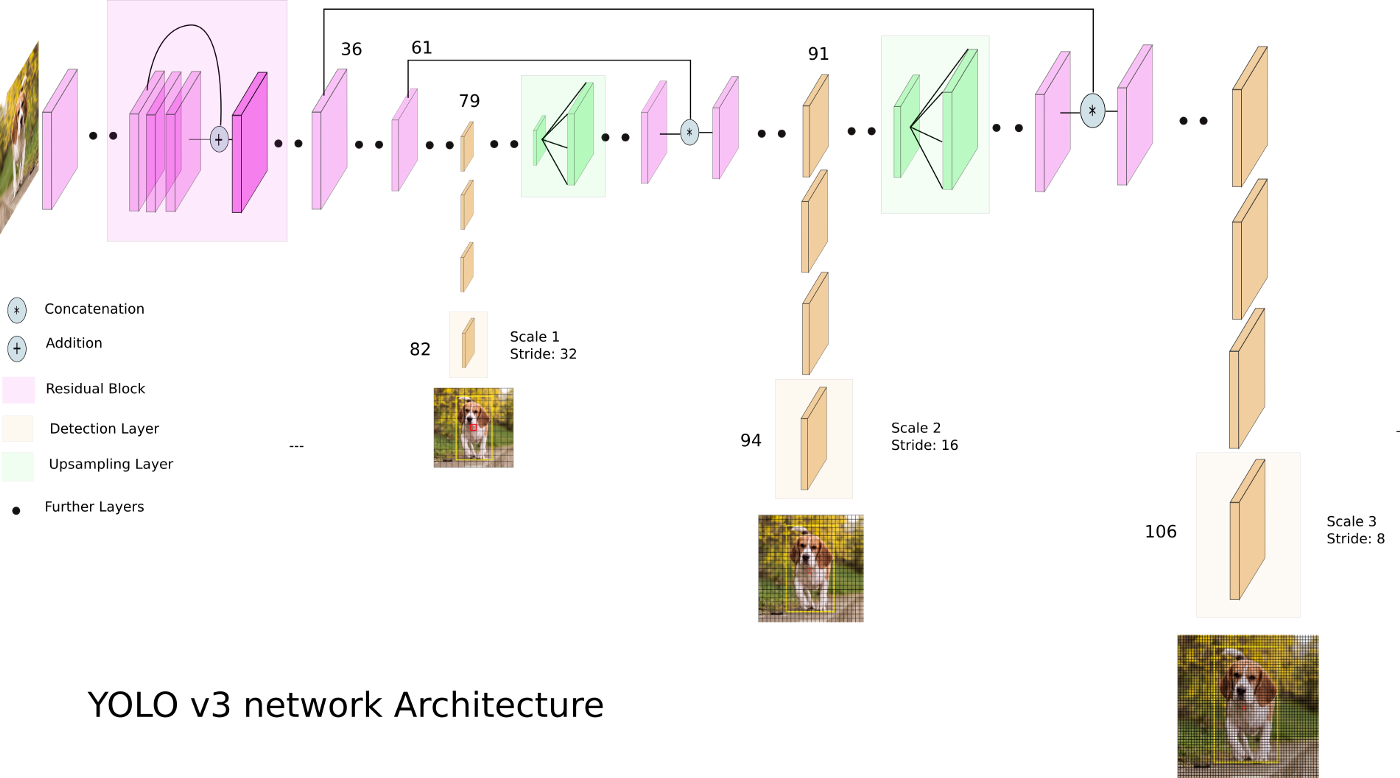
\includegraphics[scale=0.35]{figures/yolov3archi.png}
\caption{Architecture Yolov3}
\end{center}
\end{figure}
image libre de droit 
src : https://towardsdatascience.com/yolo-v3-object-detection-53fb7d3bfe6b
\\
L’IoU – ou Intersection over Union – est un indicateur de la qualité de la détection d’un objet en comparant, dans un dataset d’entraînement, la position connue de l’objet dans l’image avec la prédiction faite par l’algorithme. L’IoU est le rapport entre la surface de l’intersection de 2 bounding box (celle prédite et la véritable) considérées et la surface de l’union des 2.
\\
L’IoU peut valoir entre 0 (pour une détection totalement ratée) et 1 (pour une détection parfaite). De façon générale l’objet est considéré comme étant détecté à partir d’un IoU supérieur à un certain nombre (0.24  dans la littérature).

\\
Nous utiliserons abondamment une métrique très similaire à l'IOU comme mesure pour notre validation lors de l'entrainement. La métrique mAP basé sur la moyenne des précision. 
Pour cette première tâche nous optons pour la version3 de l'algorithme.
\\
\begin{figure}[H]
\begin{center}
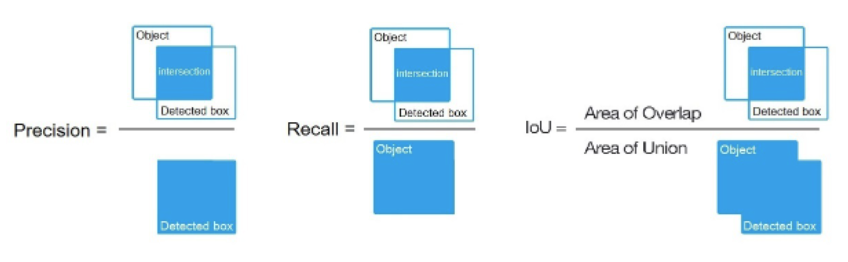
\includegraphics[scale=0.44]{figures/iou.png}
\caption{Precision - Recall - IOU src:\cite{gitlink}}
\end{center}
\end{figure}
\\
Plus de détail sur le papier de recherche de \href{https://arxiv.org/pdf/1506.02640.pdf}{YOLO.}\cite{yolopaper}

\paragraph{Premiers prétraitements}
\\
Nous avons choisi LabelImg pour annoter nos données. L'étape de l'annotation est une étape cruciale et a un impact immense sur la qualité des résultats de prédiction. Cette étape consiste à tracer des rectangles autour de l'objet que nous souhaitons détecter et d'annoter un nom de classe à chaque rectangle tracés sur l'image. Pour constituer notre jeu d'entraînement nous avons donc choisi dans un premier temps de tracer les box autour de la baleine entière sur environ 500 images. Nous verrons plus tard que c'était d'une mauvaise idée. 
\\Le logiciel génère pour chaque image un fichier txt correspondant ou chaque ligne correspond à un rectangle avec comme paramètre respectivement:
\\classe_{id}, x_{center}, y_{center}, h_{box}, w_{box}

\begin{figure}[H]
\begin{center}
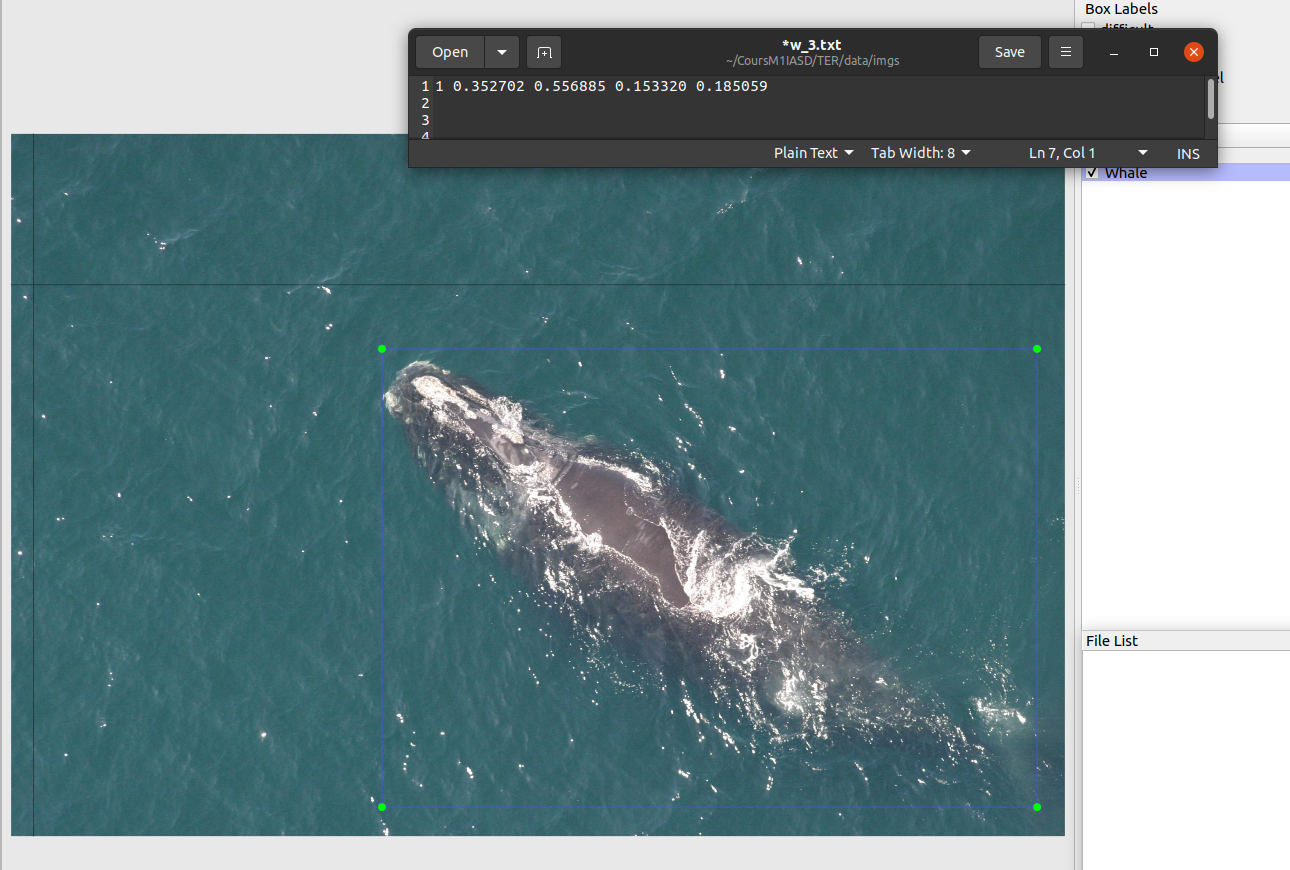
\includegraphics[scale=0.4]{figures/labelimg.png}
\caption{Labelimg - Whole whale Box}
\end{center}
\end{figure}

\paragraph{Développement du premier modèle} 
\\
Pour mettre en place un entraînement Yolo il est nécessaire de faire quelques réglages avant. Pour toutes les implémentations de l’algorithme Yolo nous avons utilisé le repo suivant\footnote{https://github.com/AlexeyAB/darknet}.
\\
Ci-dessous sont décrites les étapes effectuées dans les grandes lignes même s'il y a eu beaucoup d'étapes intermédiaires:

\begin{enumerate}
    \item \textbf{Cloner le repository}
    \item \textbf{Faire quelques changement dans le Makefile}
    Dans les lignes suivantes nous précisons que nous utiliserons les fonctionnalités pour le GPU et OpenCV.
    \begin{lstlisting}
    sed -i 's/OPENCV=0/OPENCV=1/' Makefile
    sed -i 's/GPU=0/GPU=1/' Makefile
    sed -i 's/CUDNN=0/CUDNN=1/' Makefile
    \end{lstlisting}
    Puis compiler.
    
    \item \textbf{Ajout des fichiers de configurations}
    Ajout des fichiers obj.names précisant le nom de(s) la(es) classe(s). et obj.names indiquant le chemin du fichier train.txt, le chemin d'accès au fichier d'accès au test.txt, le chemin d'accès au fichier 
    \begin{lstlisting}
    mkdir training
    echo "Whale" > data/obj.names
    echo -e 'classes= 1\ntrain  = data/train.txt\nvalid  = data/test.txt\nnames = data/obj.names\nbackup = training/' > data/obj.data
    mkdir data/obj
    \end{lstlisting}
    
    \item \textbf{Décompresser les images}
    Décompresser les images et les mettre dans le répertoire data.
    
    \item \textbf{Créer un jeu de données d'entrainement et de validation}
    à partir de toutes les images, créer un script bash (le script est disponible sur notre github) qui va diviser le jeu de manière à avoir 10\% de validation et le reste pour l'entrainement. Creer les fichier train.txt et test.txt avec la liste des chemins d'accès des images des jeux respectifs.
    
    \item \textbf{Modifier le fichier yolov3-custom.cfg}
    Modifier le fichier du paramétrage du réseau: Régler la batch size (nombre d'image envoyé par paquet durant l'entraînement). Régler la subdivision assez haute mais pas supérieur à la batch size. Attention pour ce dernier un nombre trop faible va inévitablement faire crasher le programme car il n'y aura plus assez de RAM disponible. L'entraînement de Yolo est très coûteux en ressources donc un bon conseil serait de garder le nombre de subdivisions supérieur à 32. Vient ensuite la modification du nombres de classes puis la modification de la taille des filtres à modifier sur chaque couches de sorties du réseau.
    \begin{lstlisting}
    sed -i 's/batch=1/batch=64/' cfg/yolov3_training.cfg
    sed -i 's/subdivisions=1/subdivisions=32/' cfg/yolov3_training.cfg
    sed -i 's/max_batches = 500200/max_batches = 4000/' cfg/yolov3_training.cfg
    sed -i '610 s@classes=80@classes=1@' cfg/yolov3_training.cfg
    sed -i '696 s@classes=80@classes=1@' cfg/yolov3_training.cfg
    sed -i '783 s@classes=80@classes=1@' cfg/yolov3_training.cfg
    sed -i '603 s@filters=255@filters=18@' cfg/yolov3_training.cfg
    sed -i '689 s@filters=255@filters=18@' cfg/yolov3_training.cfg
    sed -i '776 s@filters=255@filters=18@' cfg/yolov3_training.cfg
    \end{lstlisting}
    
    \item \textbf{Récuperer les poids}
    \begin{lstlisting}
    wget https://pjreddie.com/media/files/darknet53.conv.74
    \end{lstlisting}
    
    \item \textbf{Lancer l'entrainement}
    \begin{lstlisting}
    ./darknet detector train data/obj.data cfg/yolov3_training.cfg darknet53.conv.74 -dont_show -map
    \end{lstlisting}
    
\end{enumerate}

Plus de détail sur les réglages à effectuer dans le README du projet.
\paragraph{Évaluation des résultats}
\\
Malheureusement pour ce premier réseau, la trace de la métrique mAP durant l'entraînement est absente pour une raison très simple: C’était pour nous la première implémentation de l’algo YOLO, nous n’avons donc pas correctement appliqué le tuto précédent et nous avons oublié le set de validation (grosse erreur) durant l'entraînement du modèle donc impossible de garder trace des performances de notre algorithme durant l’entraînement. Pour l'évaluation de nos résultats nous avons donc simplement regardé les sorties données par l'algorithme. Les images croppées sont plutôt bonnes même si le nombre de 500 images semble un peu léger pour une détection optimale.
ex de sortie après crop de l'image sur les box prédites.
\begin{figure}[H] % "[t!]" placement specifier just for this example
\begin{subfigure}{0.45\textwidth}
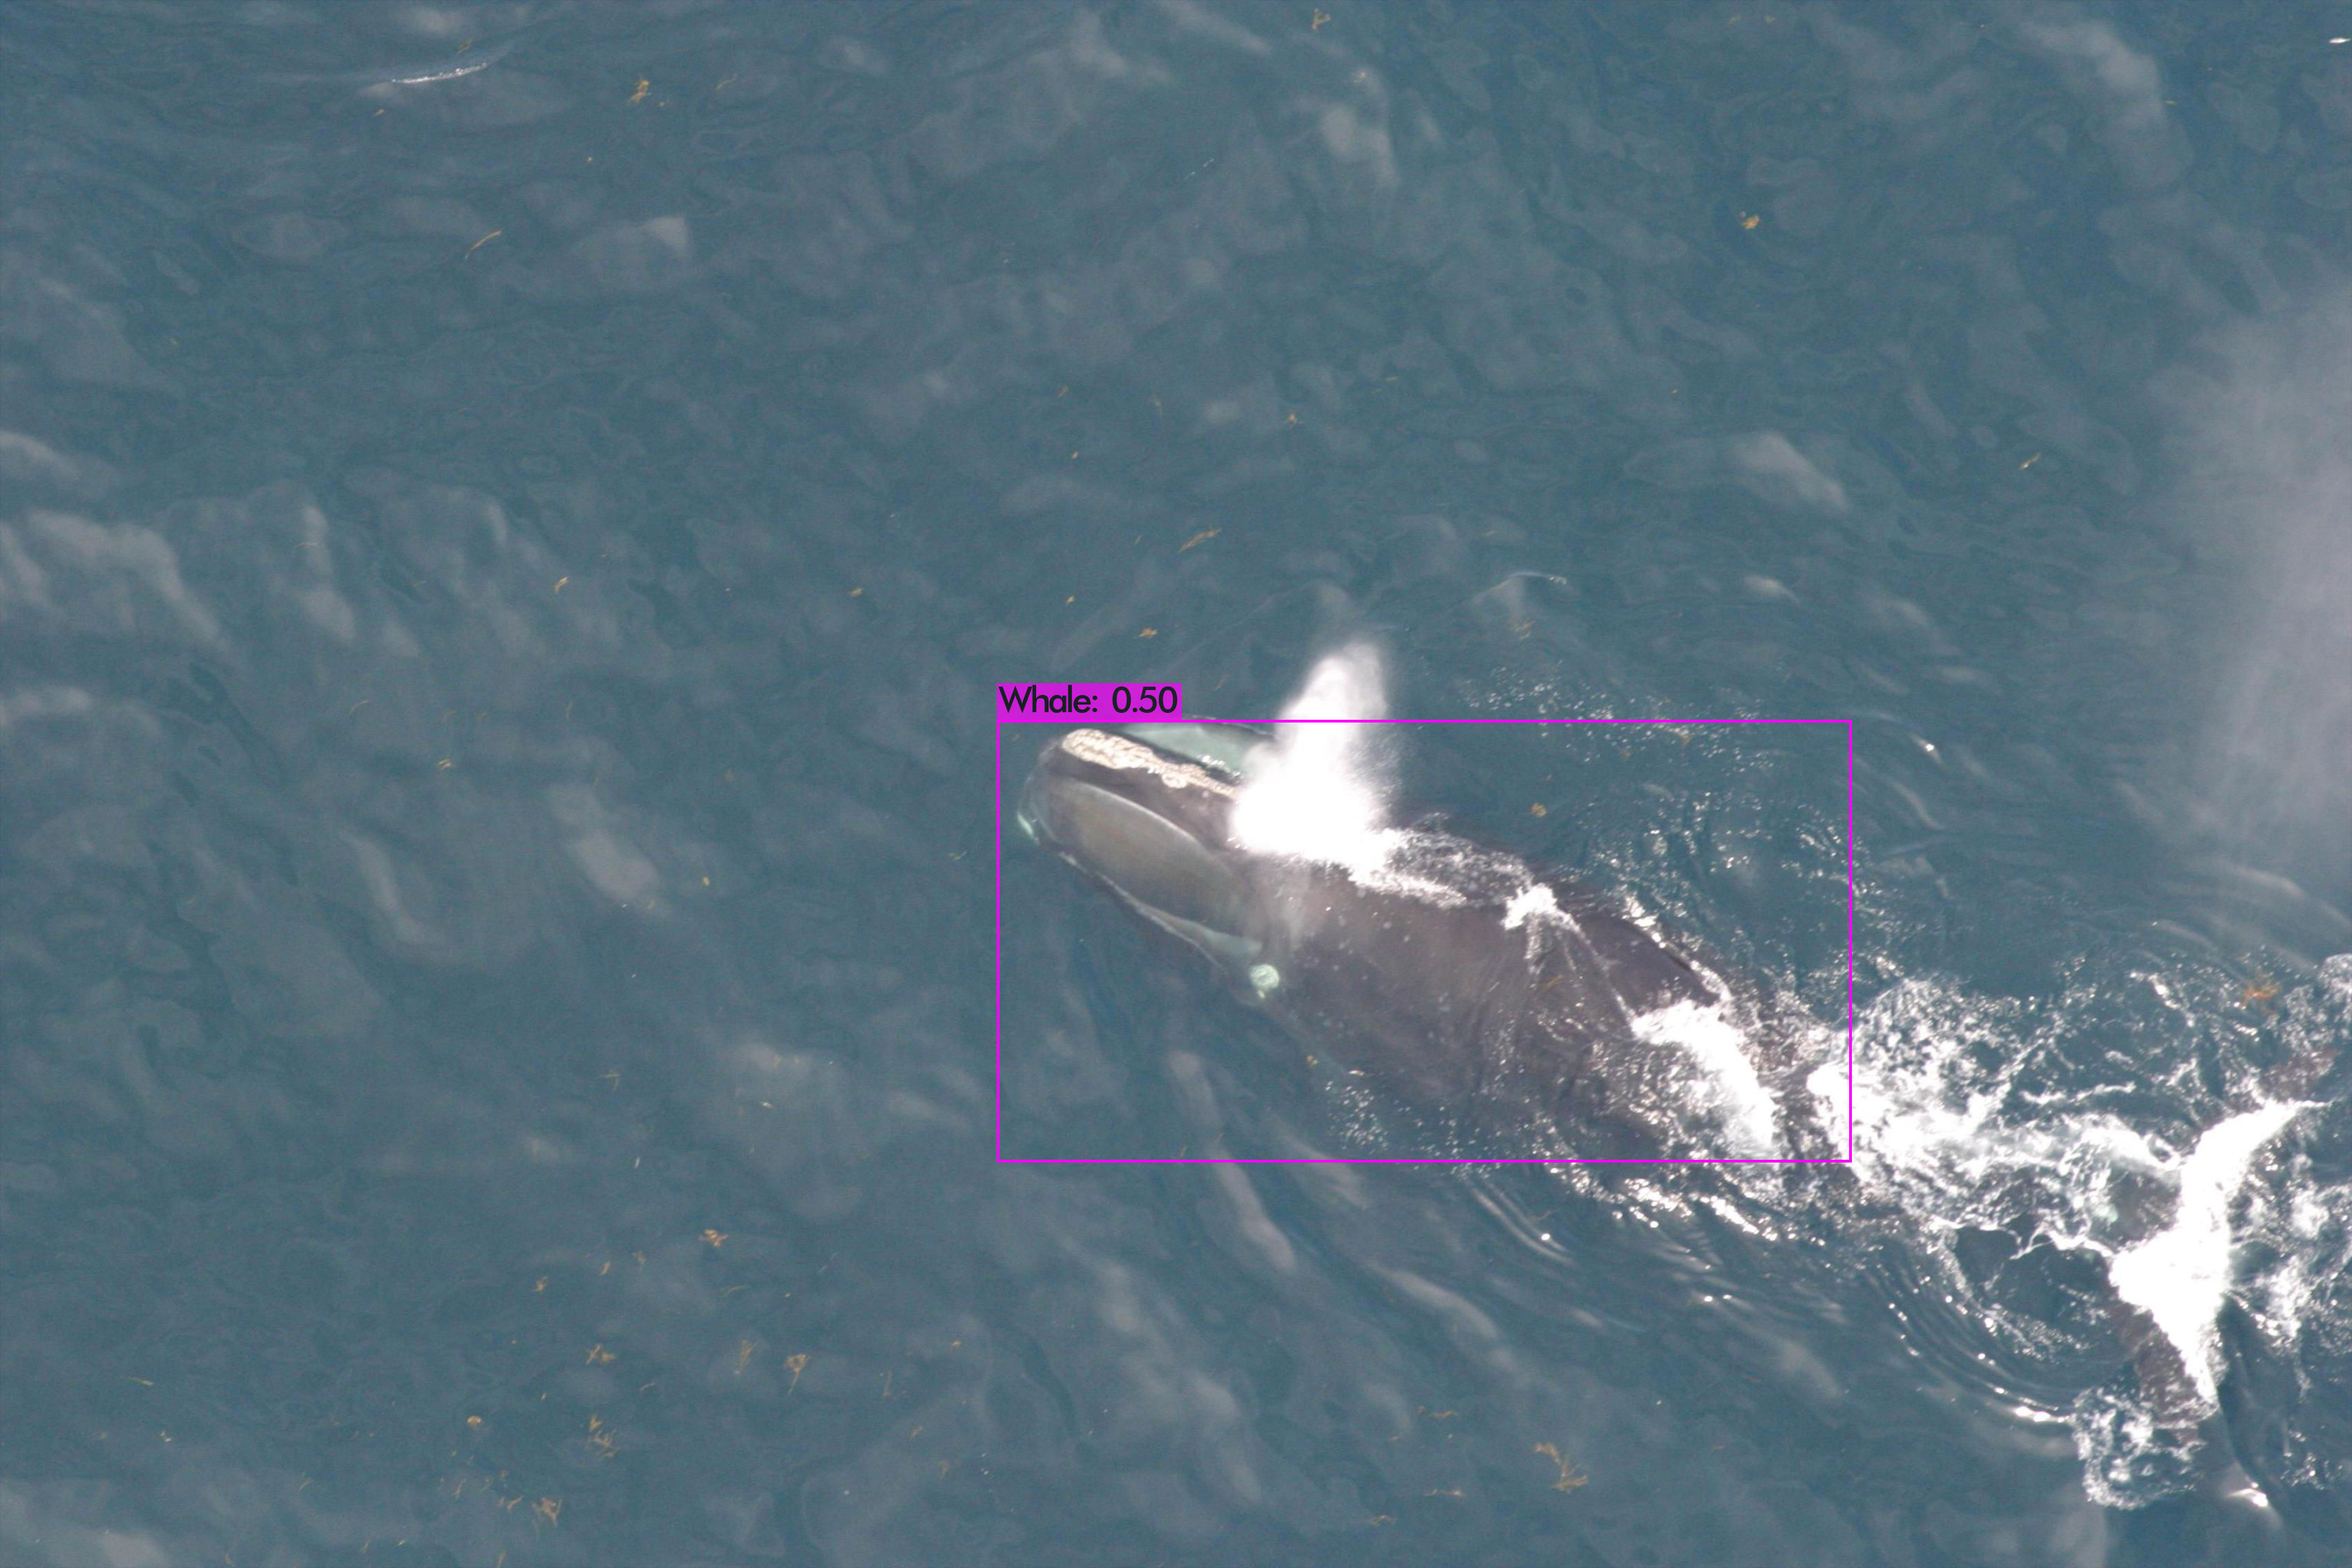
\includegraphics[width=\linewidth]{figures/sortie/yolov3/predictionsall1.jpg}
\end{subfigure}\hspace*{\fill}
\begin{subfigure}{0.45\textwidth}
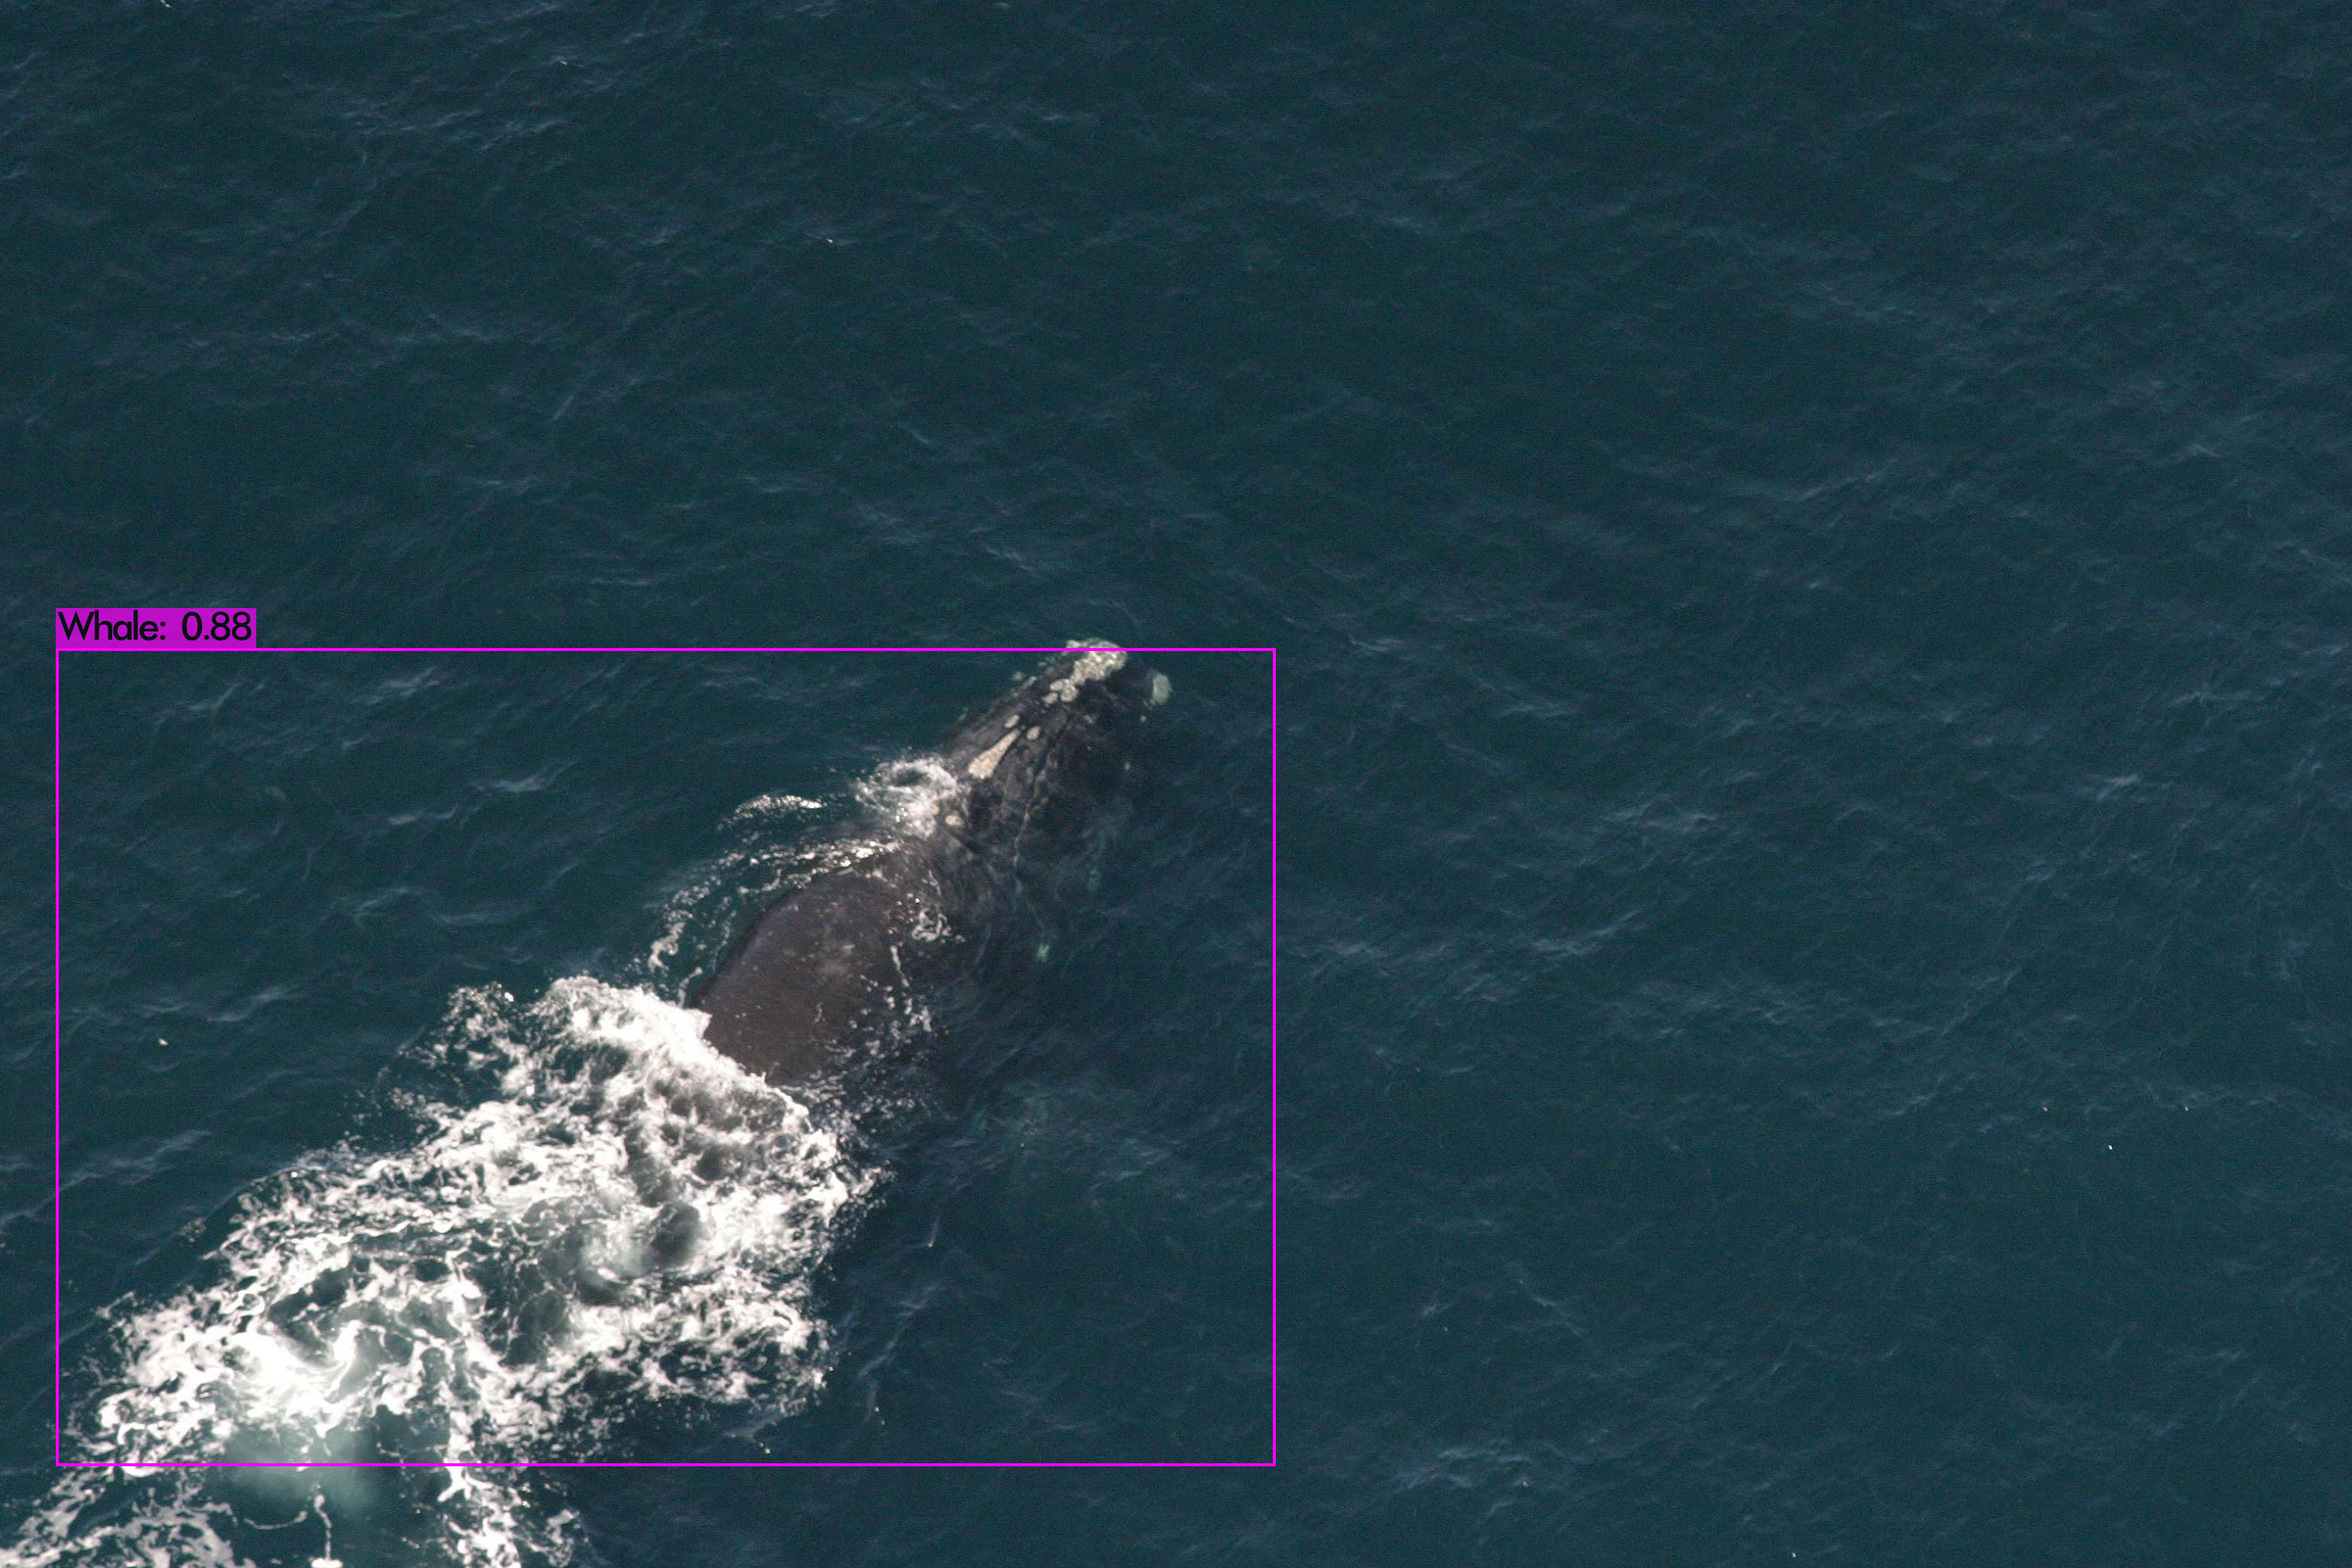
\includegraphics[width=\linewidth]{figures/sortie/yolov3/predictionsall2.jpg}
\end{subfigure}
\caption{exemple de sortie sur Yolov3}
\end{figure}

\paragraph{Problèmes et seconds prétraitements}\mbox{}\\
\\
Après, quelques recherches sur Internet sur les baleines noires on s'aperçoit que la caractéristique la plus distinctive d'une baleine noire se situe au niveau de sa tête. Les plaques rugueuses de la peau sur sa tête qui apparaissent blanches en raison du parasitisme par les poux de baleine. Il s'avère que cela les distingue non seulement des autres espèces de baleines, mais constitue également un bon moyen de différencier les individus. La solution présentée précédemment ne se concentre pas assez sur la tête mais considère la baleine entière. On décide donc d'utiliser une autre configuration: On va répéter le processus précédent mais en se concentrant uniquement sur la zone autour de la tête et de la partie haute du dos.
Nous constituons cette fois-ci un jeu de donnés d'entraînement de 3000 images.
\\
\begin{figure}[H] % "[t!]" placement specifier just for this example
\begin{subfigure}{0.45\textwidth}
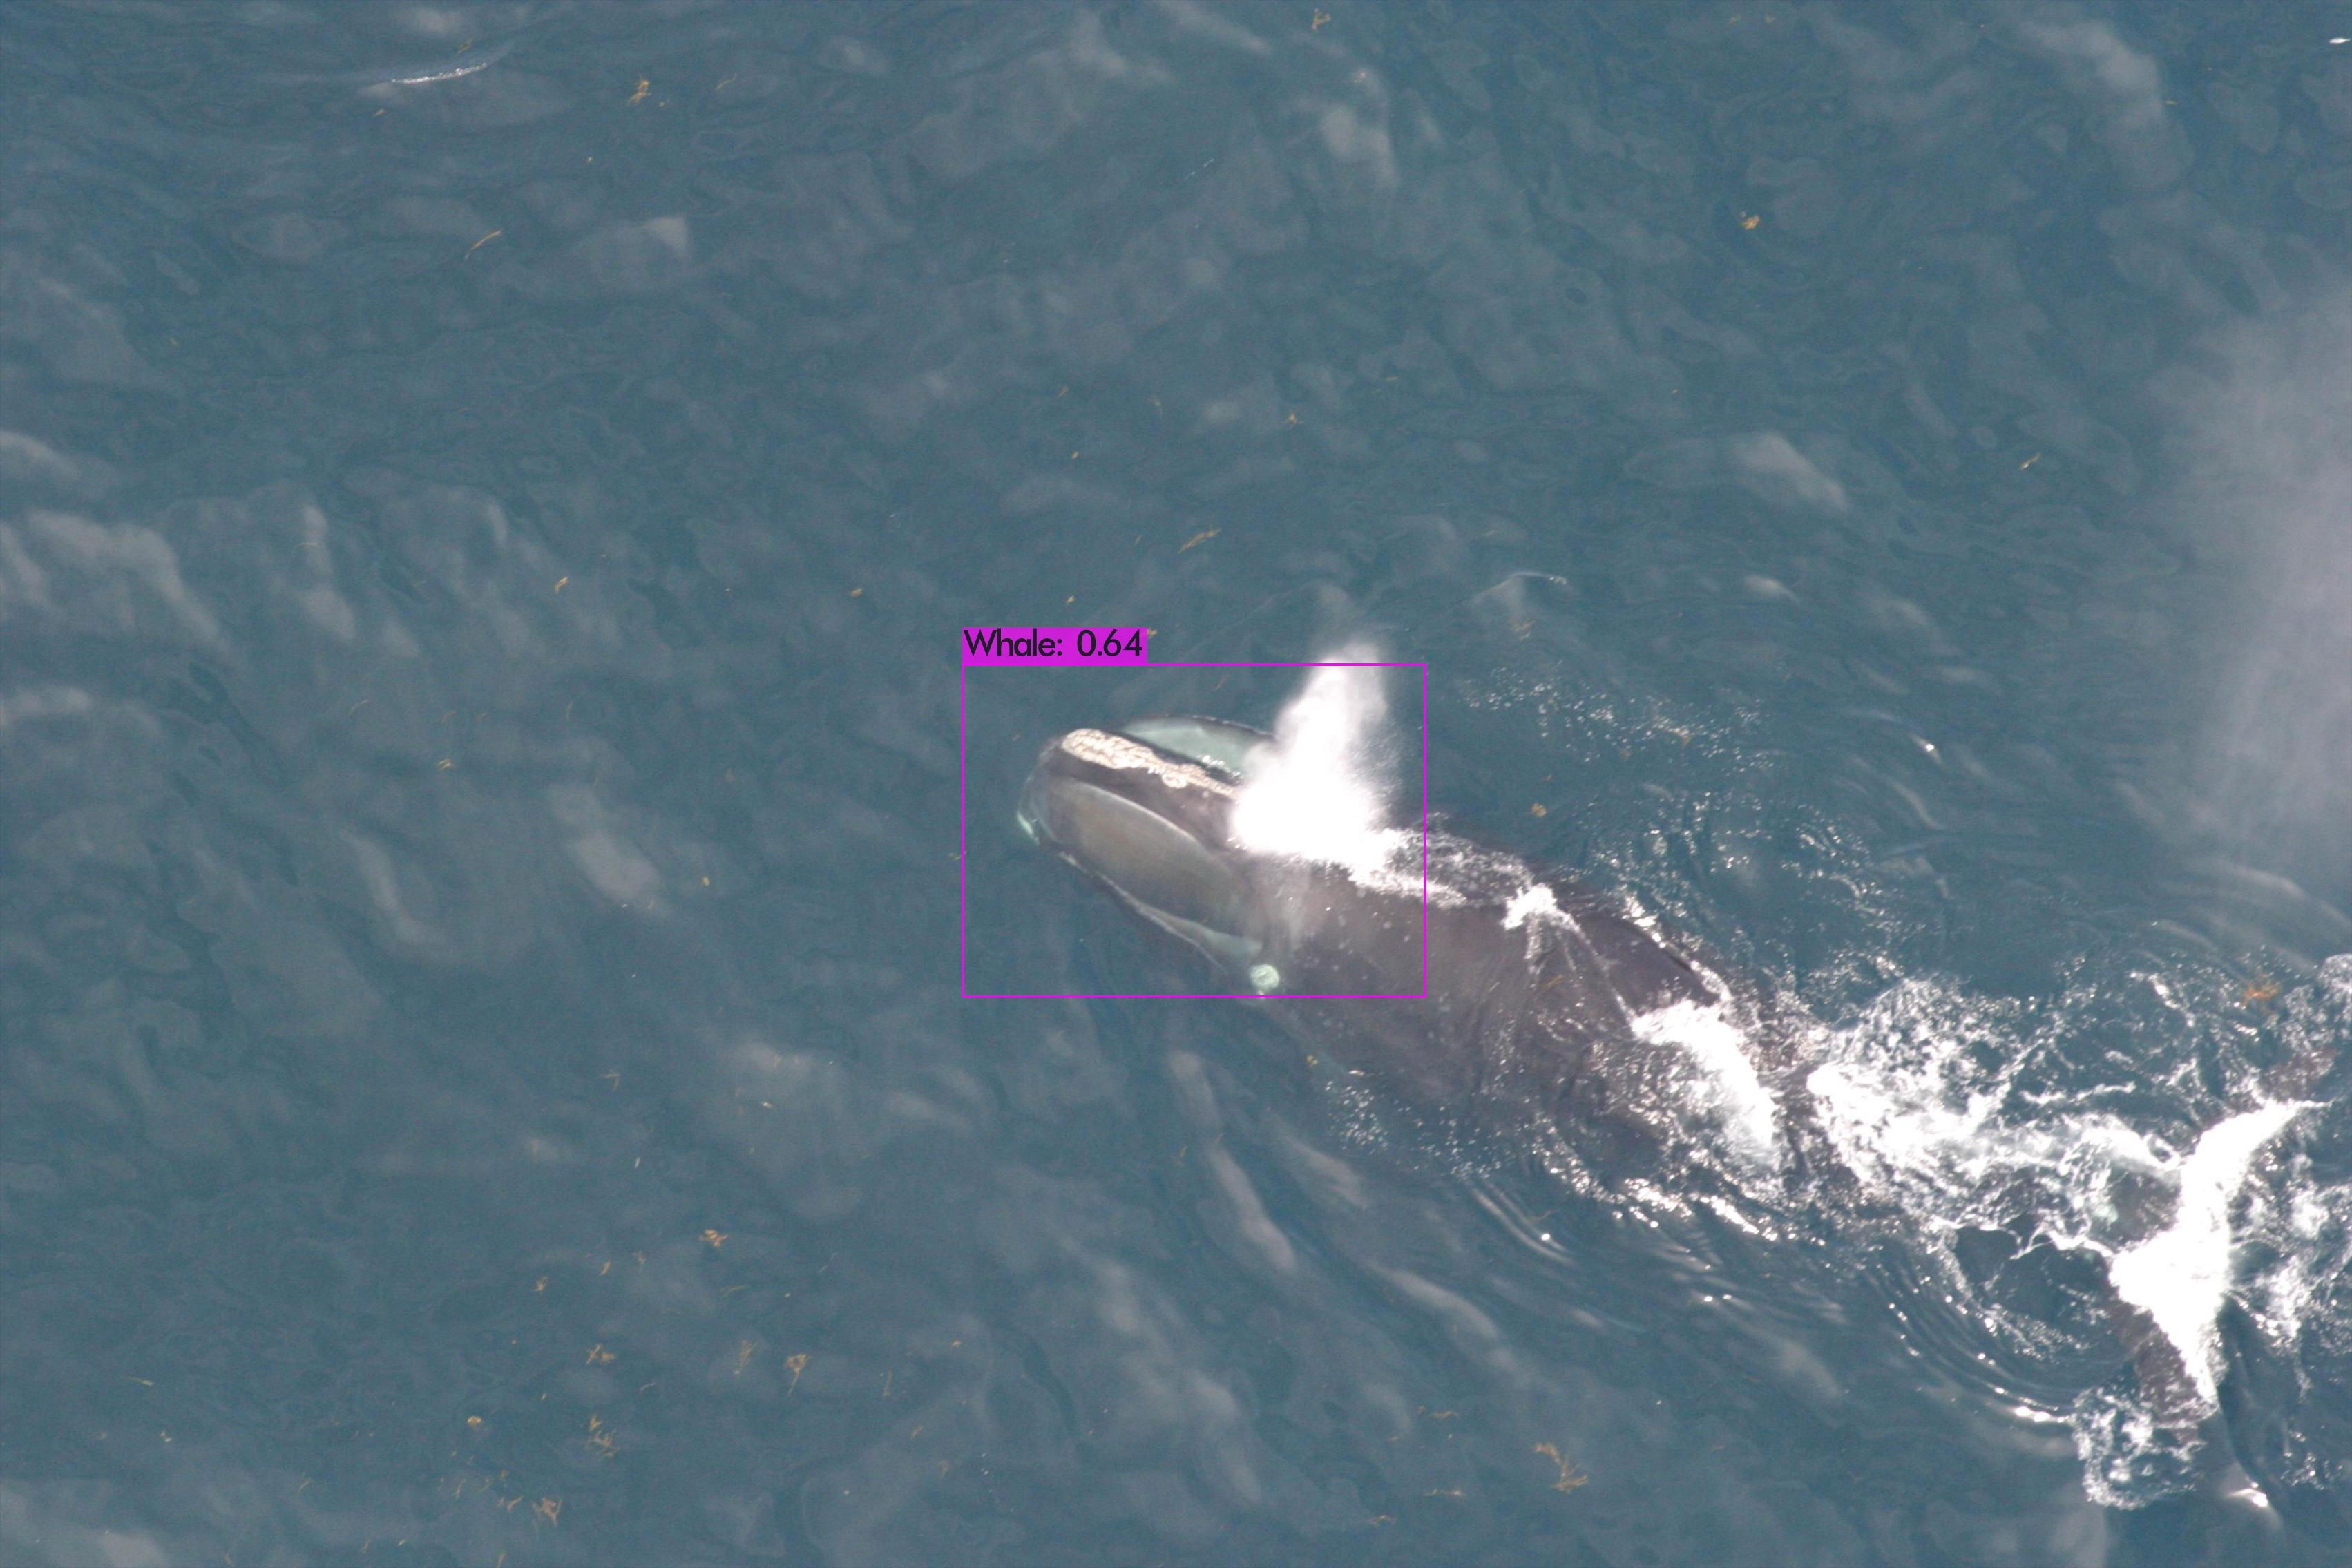
\includegraphics[width=\linewidth]{figures/sortie/yolov3/predictionshead1.jpg}
\end{subfigure}\hspace*{\fill}
\begin{subfigure}{0.45\textwidth}
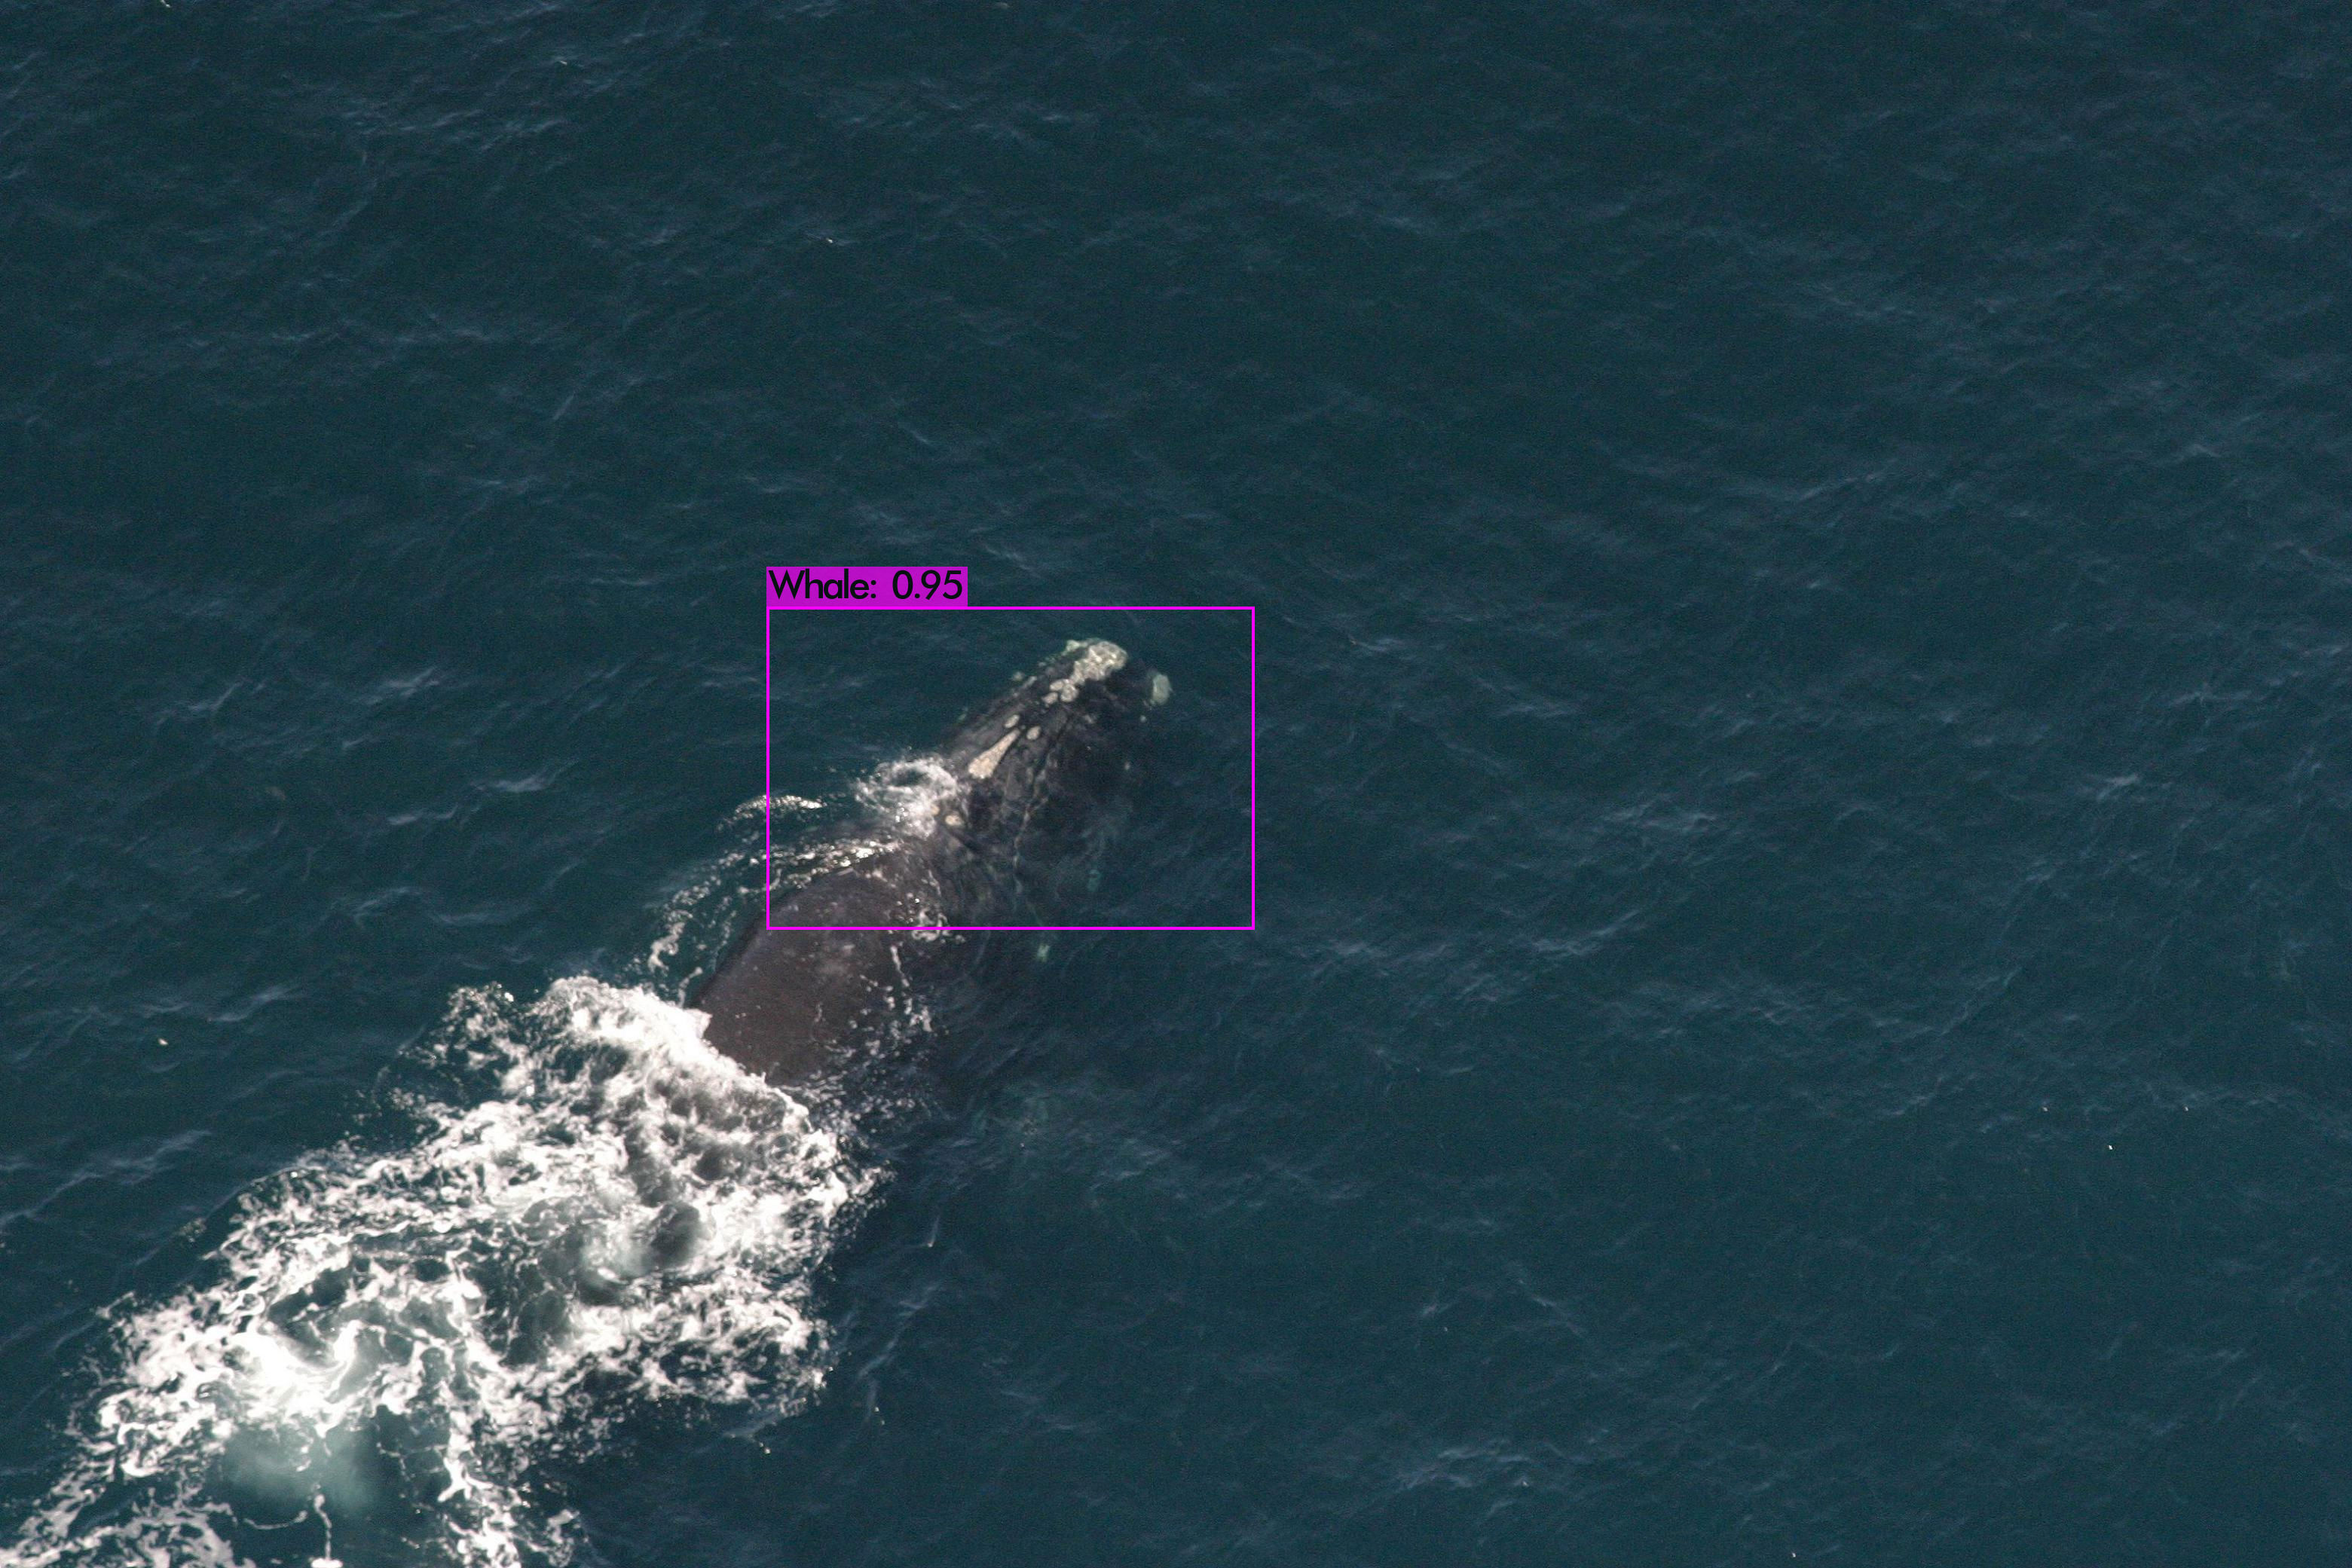
\includegraphics[width=\linewidth]{figures/sortie/yolov3/predictionshead2.jpg}
\end{subfigure}
\caption{exemple de sortie sur Yolov3 avec seulement la tête}
\end{figure}
\\
Après entraînement en appliquant cette fois ci correctement toutes les étapes, les résultats sont très bons, ci-dessous le graphique de l'entraînement n'indique pas de signe d'overfitting y compris après un temps très long. On remarque une très bonne précision d'environ 99\% (d'indice mAP ce qui n'est pas rare avec YOLO pour les gros objets), du modèle ce que nous avons pu aussi constater sur les photos. Nous avons utilisé 10\% du dataset pour la validation.
\\
\newpage

\begin{figure}[H]
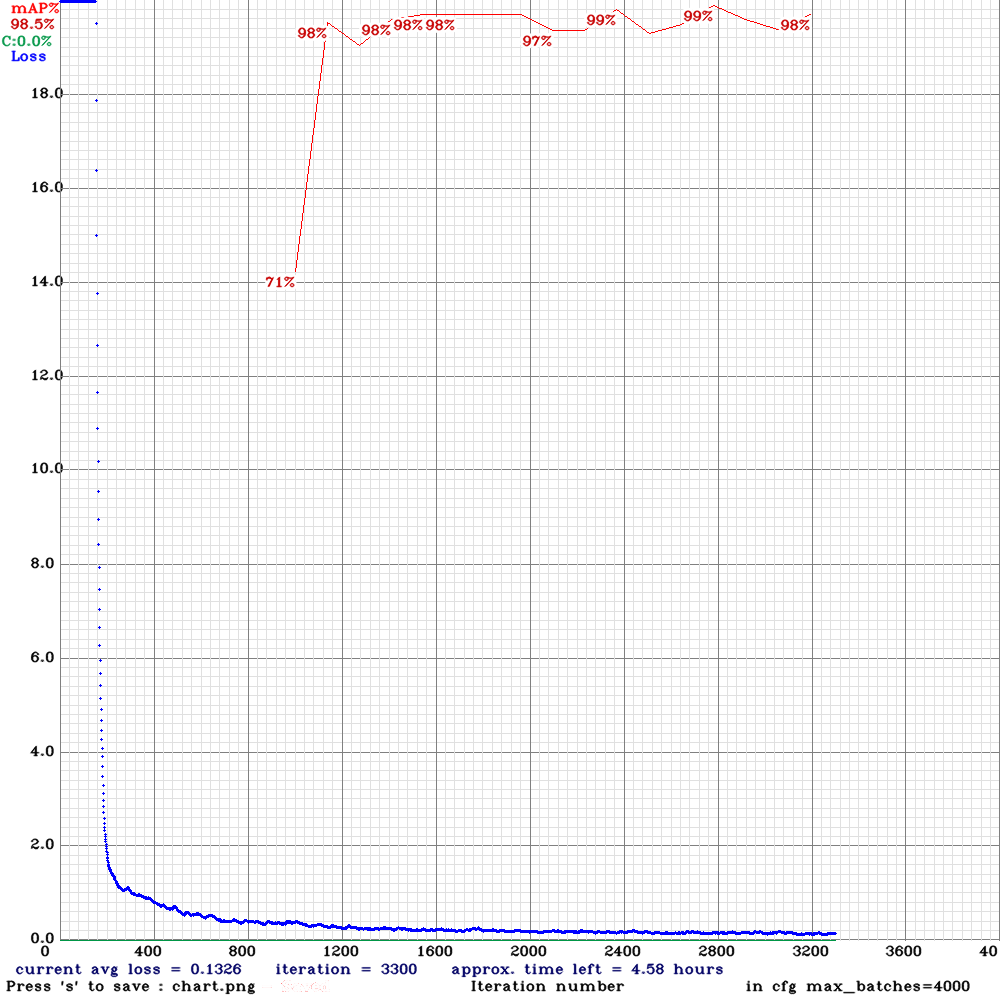
\includegraphics[scale=0.44]{figures/sortie/yolov3/chart_yolov3_training.png}
\caption{Loss et mAP pendant l'entrainement de Yolov3}
\end{figure}\\

\newpage
\subsubsection{Head Aligner Yolo v4 et Algo d'Alignement}
Une fois la partie avant de la baleine détectée, la tâche suivante consiste maintenant à aligner nos images sur un même standard de manière à constituer des sortes de photos d'identité de baleines. Cette partie est absolument primordiale à l'obtention de bons résultats lors du déroulement du 3ème algorithme qui porte sur la detéction de face. 
\\
Pour mettre en place cet alignement nous avons d’abord envisagé d’utiliser deux approches une première en essayant d’appliquer directement des opérations comme des homographies par exemple. Cette approche marche très bien dans certaines tâches de computer vision lorsqu’une sorte template de référence sert de base pour les images à aligner. Or ici ce n’est pas du tout le cas, les baleines ne se ressemblent pas toutes entre elles et les prises de vues comportent trop d’écart pour espérer qu’une approche comme celle-ci marche. 
\\Nous allons donc réutiliser l’algorithme Yolo mais cette fois-ci dans sa version 4 qui est plus performante dans la détection de petits objets. Nous utiliserons 2 classes: une classe Head(rectangle tracé autour de la tête) et une classe Air (rectangle tracé autour de l’évent).

\paragraph{Premiers prétraitements} \mbox{}\\


\paragraph{Développement du second modèle}\mbox{}\\

\paragraph{Résultats}\mbox{}\\


\begin{figure}[H] % "[t!]" placement specifier just for this example
\begin{subfigure}{0.56\textwidth}
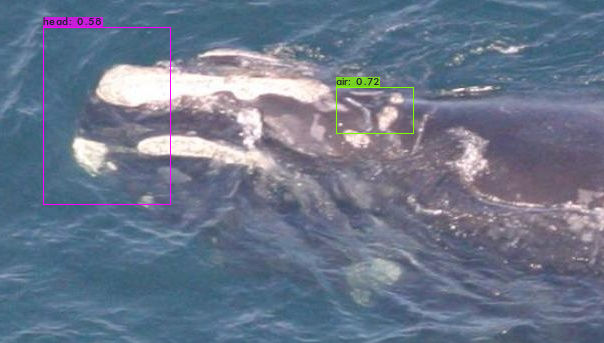
\includegraphics[width=\linewidth]{figures/sortie/yolov4/predictions1.jpg}
\end{subfigure}\hspace*{\fill}
\begin{subfigure}{0.5\textwidth}
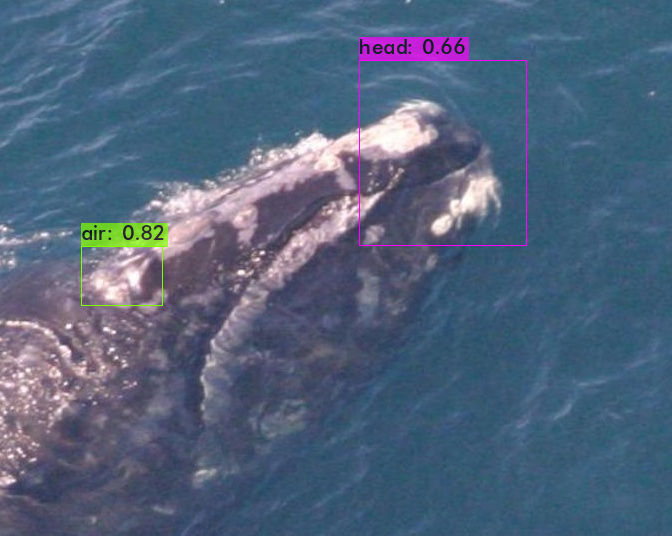
\includegraphics[width=\linewidth]{figures/sortie/yolov4/predictions2.jpg}
\end{subfigure}
\medskip
\begin{subfigure}{0.55\textwidth}
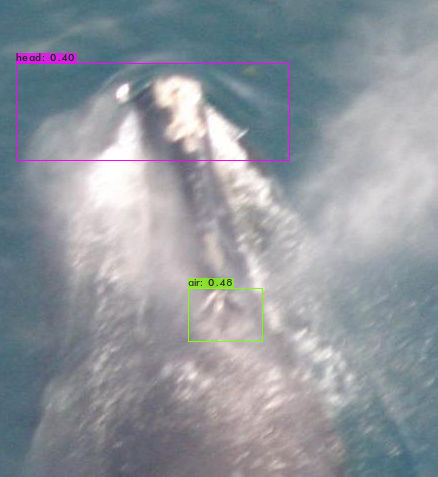
\includegraphics[width=\linewidth]{figures/sortie/yolov4/predictions3.jpg}
\end{subfigure}\hspace*{\fill}
\begin{subfigure}{0.58\textwidth}
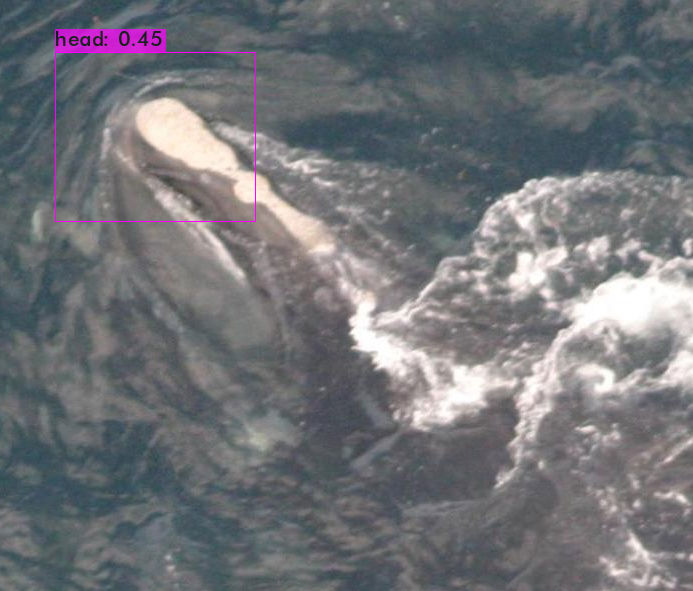
\includegraphics[width=\linewidth]{figures/sortie/yolov4/predictions4.jpg}
\end{subfigure}
\caption{Résultat Yolov4 sur les attributs} \label{fig:1}
\end{figure}

blalbla

\begin{figure}[H]
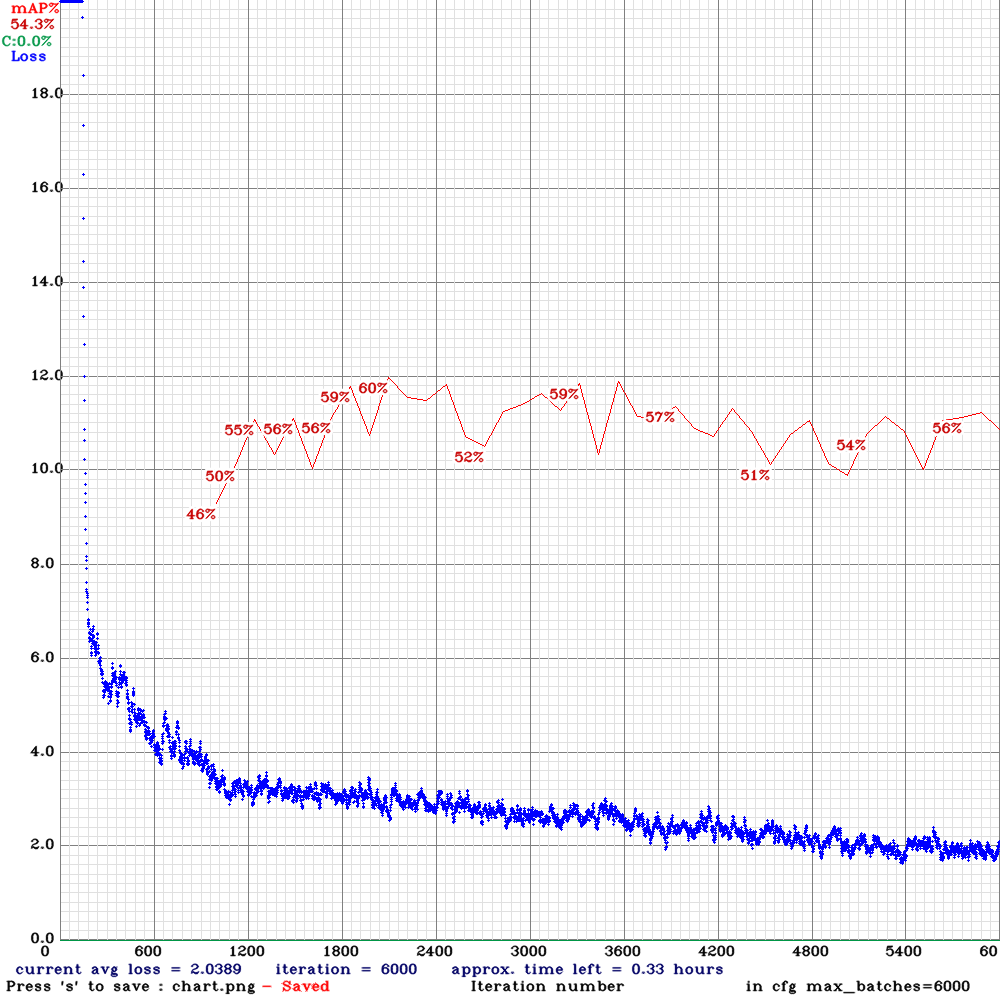
\includegraphics[scale=0.44]{figures/sortie/yolov4/chart.png}
\caption{Loss et mAP pendant l'entrainement de Yolov3}
\end{figure}\\


\paragraph{Alignement des images}\mbox{}\\
\newpage
\subsubsection{Système de reconnaissance faciale}
\newpage
\paragraph{Premiers prétraitements} \mbox{}\\
\newpage
\paragraph{Développement du second modèle}\mbox{}\\
\newpage
\paragraph{Résultats}\mbox{}\\
\newpage

\newpage
\paragraph{Alignement des images}\mbox{}\\
\newpage
\section{Conclusion}

\begin{spacing}{1.5}
\subsection{Perspectives d'amélioration}


\subsection{Ce qu'on a appris}


\end{spacing}

\cleardoublepage
\addcontentsline{toc}{chapter}{Bibliographie}
\bibliographystyle{plain}
\bibliography{Bibliographie}

\end{document}
